%Version 3.1 December 2024 -- Springer Nature LaTeX template (sn-jnl)
%% Reference style: sn-basic without "Numbered" = Springer Basic author-year citations,
%% as required by Virtual Reality ("Cite references in the text by name and year in parentheses").
\documentclass[pdflatex,sn-basic]{sn-jnl}

\usepackage{graphicx}%
\usepackage{multirow}%
\usepackage{amsmath,amssymb,amsfonts}%
\usepackage{amsthm}%
\usepackage{mathrsfs}%
\usepackage[title]{appendix}%
\usepackage{xcolor}%
\usepackage{textcomp}%
\usepackage{manyfoot}%
\usepackage{booktabs}%
%% hyperref and natbib are loaded by sn-jnl.cls, so \autoref, \citet and \citep work without extra packages.

\raggedbottom

\begin{document}

\title[Stress and Interaction in Virtual Reality]{Measuring the Effects of Stress on Interaction in Virtual Reality}

%% Corresponding author is marked with \author*; change it if needed.
\author[1]{\fnm{Guangzheng} \sur{Zhang}}\email{gzha0016@uni.sydney.edu.au}
\author[1]{\fnm{Shakyani} \sur{Jayasiriwardene}}\email{djay0399@uni.sydney.edu.au}
\author[1]{\fnm{Zheyuan} \sur{Kuang}}\email{zkua0021@uni.sydney.edu.au}
\author[1]{\fnm{Tinghui} \sur{Li}}\email{tili4998@uni.sydney.edu.au}
\author[2]{\fnm{Jonathan} \sur{Bird}}\email{j.m.bird@ucl.ac.uk}
\author[3]{\fnm{Nicholas} \sur{Koemel}}\email{nicholas.koemel@sydney.edu.au}
\author[3]{\fnm{Matthew} \sur{Ahmadi}}\email{matthew.ahmadi@sydney.edu.au}
\author[2]{\fnm{Mark} \sur{Hamer}}\email{m.hamer@ucl.ac.uk}
\author[3]{\fnm{Emmanuel} \sur{Stamatakis}}\email{emmanuel.stamatakis@sydney.edu.au}
\author[4]{\fnm{Weiwei} \sur{Jiang}}\email{weiweijiangcn@gmail.com}
\author[1]{\fnm{Anusha} \sur{Withana}}\email{anusha.withana@sydney.edu.au}
\author*[1]{\fnm{Zhanna} \sur{Sarsenbayeva}}\email{zhanna.sarsenbayeva@sydney.edu.au}

%% TODO: fill in each \orgdiv (school/department). [3] is a separate entry in case these co-authors are in a different school.
\affil[1]{\orgdiv{School of Computer Science}, \orgname{The University of Sydney}, \orgaddress{\city{Sydney}, \state{NSW}, \country{Australia}}}
\affil[2]{\orgdiv{XXX}, \orgname{University College London}, \orgaddress{\city{London}, \country{UK}}}
\affil[3]{\orgdiv{XXX}, \orgname{The University of Sydney}, \orgaddress{\city{Sydney}, \state{NSW}, \country{Australia}}}
\affil[4]{\orgdiv{XXX}, \orgname{Nanjing University of Information Science and Technology}, \orgaddress{\city{Nanjing}, \country{China}}}

%% Journal limit: 150--250 words (this version: 234 words).
\abstract{Acute stress can affect cognition and interaction performance, but it remains unclear whether stress acts as a general impairment in immersive interaction or whether its effects depend on the demands of the task. We investigated how acute stress influences three interaction tasks in virtual reality (VR): target acquisition, reading aloud, and the Tower of London. In a within-subject study, 24 participants (11 female, 13 male; aged 20--31 years) completed the tasks at baseline, after a VR-based Trier Social Stress Test (VR-TSST), and after a recovery period. Stress induction increased state anxiety and heart rate and reduced heart rate variability during the VR-TSST. In the subsequent task rounds, movement time, throughput, and endpoint offset in target acquisition did not differ across phases. In reading aloud, mean fundamental frequency rose by 5.55~Hz (about 3\%), whereas speech timing was unchanged. In the Tower of London task, planning measures were unchanged,  whereas execution time was 36\% shorter after induction. Although state anxiety remained elevated at the end of the post-stress round, heart rate during the VR tasks did not differ from the baseline round. These findings indicate that acute stress did not produce a general decline in VR interaction performance in the minutes after induction, that its behavioural traces were subtle, and that assessing stress in VR depends on what the user is doing when it is measured.}

%% Journal limit: 4--6 keywords.
\keywords{acute stress, virtual reality, situational impairments, target acquisition, reading aloud, Tower of London}

\maketitle

% \section{Introduction}
\section{Introduction}
% the world
Immersive systems are increasingly used for remote operation~\citep{haidegger2011surgery}, simulation-based training~\citep{radianti2020systematic}, and social interaction~\citep{li2021social,wei2022communication}. In these settings, stress may arise from task demands~\citep{arora2010stress} or be deliberately induced in training~\citep{kleygrewe2024virtual}, social-evaluative scenarios~\citep{helminen2019metaanalysis}, and exposure therapy~\citep{carl2019virtual}. Prior research suggests that stressful immersive experiences can affect users' physiological responses~\citep{vandammen2022evoking}, speech~\citep{dillon2021real}, and task performance~\citep{peterson2018effects}. Understanding how acute stress is reflected in movement, speech, and task timing can inform the evaluation and design of VR interaction.
%big but
Immersive tasks often combine visual attention, manual control, speech production, working memory, and planning. A single measure of overall performance gives limited insight into how these aspects of interaction change. Several theoretical perspectives suggest that the effects of acute stress do not share a single direction. Research on stress-related disruption to prefrontal function~\citep{arnsten2009stress,qin2009acute} suggests that acute stress may affect working memory and aspects of executive control~\citep{shields2016effects}. Acute stress induced by the Trier Social Stress Test (TSST)~\citep{kirschbaum1993trier} can be accompanied by elevated state anxiety and physiological arousal~\citep{allen2014biological}. And attentional control theory~\citep{eysenck2007anxiety} distinguishes performance effectiveness from processing efficiency, suggesting that additional effort may sustain observed performance under anxiety. Attentional narrowing~\citep{easterbrook1959effect} offers another possibility: heightened emotional arousal may narrow the range of cues used, potentially benefiting performance when task-irrelevant cues are excluded. Studies of acute stress have also reported improved selectivity for task-relevant information~\citep{chajut2003selective} and increased shielding of action goals at the expense of cognitive flexibility~\citep{plessow2011inflexibly}. Together, these accounts suggest that observed performance may decline, remain stable, or improve under particular conditions. They therefore motivate examining the direction and magnitude of change in individual measures across tasks with different demands.

% thereore we did

We examine acute stress within the perspective of situationally induced impairments and disabilities (SIID) research~\citep{sears2003computers,sarsenbayeva2019measuring}. Multiple Resource Theory (MRT)~\citep{wickens2008multiple} guides the selection of three controlled probes spanning demands common in immersive interaction: target acquisition for visuomotor control, reading aloud for verbal production, and the Tower of London for executive planning (Figure~\ref{fig:mrt}). The same participants completed these tasks in one VR environment at baseline, after a VR adaptation of the Trier Social Stress Test (VR-TSST)~\citep{kirschbaum1993trier,liszio2018relaxing}, and after a recovery period. We examine each task through its own measures and baseline, alongside state anxiety and cardiovascular measurements collected across the experimental sequence.
%res
State anxiety rose after the VR-TSST, and mean HR increased and RMSSD decreased during the Induction window. In the subsequent probes, mean fundamental frequency ($F_0$) during reading aloud increased by approximately 3\%, and Tower of London execution time was shorter after induction, whereas target acquisition and Tower of London planning measures showed no phase differences. Although state anxiety remained elevated at the end of the Post-Stress round, heart rate during that round did not differ from the Baseline round.
%contribution


% Immersive systems are increasingly used for remote operation~\citep{haidegger2011surgery}, simulation-based training~\citep{radianti2020systematic}, and socially interactive environments~\citep{li2021social,wei2022communication}. In these settings, users rarely engage in a single mode of interaction. Instead, they coordinate manual control, spoken communication, and decision making within the same task. Such coordination draws on multiple, partially independent cognitive resources including processing stages, processing codes, perceptual modalities, and response modalities~\citep{wickens2008multiple} that may compete for limited capacity, and is plausibly vulnerable to disruption when users are under acute stress -- a common situational factor in real-world immersive use. Whether stress degrades VR interaction uniformly, or selectively affects components with different resource demands, remains an open question.

% Prior work on situationally-induced impairments and disabilities (SIID) has typically studied stress and task performance in non-immersive settings and on isolated tasks~\citep{sears2003computers,sarsenbayeva2019measuring}, without explicitly relating stress effects to the resource profiles of the interaction components involved. Without such a framing, it is difficult to anticipate which aspects of immersive interaction are most likely to break down under stress, or to design adaptive support for the specific component being affected, such as manual selection, speech production, or planning and execution.

% To address this, we adopt Multiple Resource Theory (MRT)~\citep{wickens2008multiple} as a task-selection framework. MRT models human performance as depending on multiple partially independent resource channels, providing a principled basis for decomposing complex VR interaction into components with distinct demand profiles (Figure~\ref{fig:mrt}). Guided by MRT, we selected three controlled tasks that recur across immersive systems: a \textit{target acquisition} task~\citep{li2025estimating} for perceptual-motor interaction, a \textit{reading aloud} task~\citep{dillon2021real} for verbal production, and a \textit{Tower of London} task~\citep{shallice1982specific} for executive planning. Rather than directly quantifying resource competition, we use these tasks as an initial empirical step toward understanding how stress modulates behaviour across different resource profiles.

% We instantiate this design in a controlled experiment using the Virtual Reality Trier Social Stress Test (VR-TSST)~\citep{liszio2018relaxing}, combining behavioural performance, speech features, and physiological responses. The results do not support a uniform degradation account. In particular, the three interaction components show distinct patterns and magnitudes of change under stress, indicating that situational impairments in VR are task-specific rather than global.

\textbf{Contributions.} (1)~We extend SIID research to immersive VR by examining acute stress across three recurring interaction tasks: target acquisition, reading aloud task, and Tower of London planning, alongside subjective and physiological stress measures. (2)~We provide a task-specific account of changes following acute stress induction, reporting the direction, magnitude, and uncertainty of movement, vocal, and planning-related measures, with exploratory analyses identified explicitly.  (3)~We draw out implications for stress-aware VR systems, arguing that adaptive support should jointly consider the user's stress state and the resource demands of the current task.

% As immersive systems are increasingly used in scenarios such as remote operation~\citep{haidegger2011surgery}, simulation-based training~\citep{radianti2020systematic}, and socially interactive environments~\citep{li2021social,wei2022communication}, users are often required to coordinate multiple forms of interaction within the same setting, including manual control, spoken communication, and decision making. Such complex interaction does not rely on a single cognitive process, but instead requires the coordination of multiple resource channels that may compete for limited capacity. Under stress, this coordination may be further disrupted, potentially leading to uneven or task-specific changes in performance rather than uniform degradation.

\begin{figure*}[!t]
    \centering
    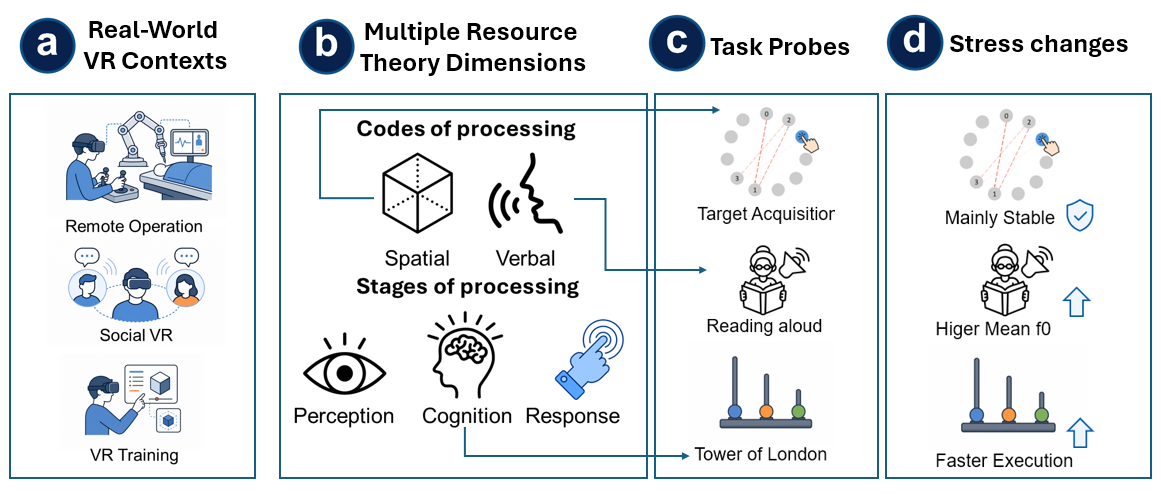
\includegraphics[width=1\textwidth]{Figure/intro.png}
    \caption{Overview of the MRT-informed task-probe approach. We decompose VR interaction demands using selected MRT dimensions and examine stress effects through target acquisition, reading aloud, and Tower of London probes.}
    \label{fig:mrt}
\end{figure*}

\section{Related work}
\label{sec:relatedwork}

\subsection{Situational Impairments and Stress in Interactive Systems}
HCI research has traditionally evaluated interaction techniques under controlled laboratory conditions, often assuming stable cognitive and physical capabilities. Real-world interaction, however, frequently occurs in dynamic contexts that temporarily disrupt these capabilities. \citet{sears2003computers} introduced the concept of situationally induced impairments and disabilities (SIID) to describe such transient limitations in otherwise able-bodied users, arising from contextual factors such as environmental conditions, multitasking, and cognitive demands. Subsequent work has refined SIID as a broad class of context-dependent disruptions affecting interaction across diverse settings~\citep{li2026survey}.

This concept has recently been extended to immersive environments, where perception, action, and feedback are tightly coupled and interaction is therefore especially sensitive to contextual variation~\citep{li2026survey}. Walking and physical encumbrance reduce interaction accuracy and movement efficiency~\citep{li2025estimating}, while ambient noise~\citep{li2025noise} and lighting conditions~\citep{liu2025understanding} affect text entry, pointing performance, and task completion time. These findings indicate that behaviour observed under controlled conditions may not generalize to real-world immersive use.

Beyond environmental and physical factors, situational contexts can induce cognitive disruptions that substantially shape interaction. Acute stress, in particular, has been shown to alter attentional control~\citep{sarsenbayeva2019measuring}, cognitive load~\citep{hou2025cognitive}, and task strategies~\citep{mcguire2023stress}. Within HCI, \citet{sarsenbayeva2019measuring} demonstrated that acute stress affects mobile target acquisition, visual search, and text entry, reducing both accuracy and completion time. Complementary work in affective HCI and motor control suggests that emotional states can modulate low-level motor behaviour: affective priming influences pointing performance under Fitts' Law paradigms~\citep{joo2026quantifying}, and anxiety or cognitive stress can alter physiological tremor and fine motor variability~\citep{budini2022mental}. This line of work, however, focuses on affective priming or single-task motor performance rather than acute social stress in immersive multi-task settings. Taken together, prior work~\citep{sarsenbayeva2019measuring, joo2026quantifying, budini2022mental} establishes that situational and affective states can influence interaction, yet how acute stress manifests in immersive environments across tasks with different cognitive and perceptual demands remains unclear.

\subsection{Inducing and Measuring Stress in Immersive Environments}
A substantial body of research has examined the effects of acute stress on cognition, showing that it impairs working memory, reduces cognitive flexibility, and disrupts executive functioning~\citep{arnsten2009stress,starcke2016effects}, as well as higher-order processes such as decision making and attentional control~\citep{qin2009acute, starcke2012decision}. Thus, stress introduces systematic changes across cognitive functions that are essential for interactive behaviour.

The Trier Social Stress Test (TSST)~\citep{kirschbaum1993trier} is one of the most widely used paradigms for inducing acute stress in controlled settings. By combining public speaking and mental arithmetic calculations under social evaluation, it reliably elicits both physiological and psychological responses. These responses unfold over time: physiological arousal rises during the stress inducement and declines afterwards, and reactivity to and recovery from the TSST are commonly examined as distinct processes~\citep{linden1997physiological,chida2008chronic}. In HCI, the TSST has been used to examine stress effects on mobile interaction, with measurable impacts on target acquisition, visual search, and text entry~\citep{sarsenbayeva2019measuring}, and on reliance decisions during interaction with automated systems~\citep{mcguire2023stress}.

Immersive environments have emerged as a complementary platform for studying stress and emotion. \citet{liszio2018relaxing, liszio2019interactive} showed that VR can both induce and regulate stress, with effects comparable to real-world TSST paradigms. Building on this, \citet{zhang2026seconds} designed a VR-based stress inoculation training system for novice physicians, identifying support strategies such as self-regulation aids, procedure guidance, and sensory support. While that work targets intervention design in a medical training scenario, our study examines how acute stress affects underlying VR interaction components, which can in turn inform when and what kinds of support are needed. Related VR affective computing research further shows that immersive scenes can elicit emotions~\citep{jiang2024immersive} and that interaction itself can modulate emotional experience~\citep{kuang2026understanding}, supporting VR as a controlled yet ecologically relevant platform for studying how stress- and emotion-related state changes unfold during interaction.

Stress is typically assessed through a combination of subjective, physiological, and behavioural measures, including self-report scales such as the State-Trait Anxiety Inventory (STAI)~\citep{spielberger1971state}, heart rate and heart-rate variability~\citep{kim2018stress}, and behavioural indicators such as completion time and error rate~\citep{li2026survey,sarsenbayeva2019measuring}. Together, these measures capture both internal state changes and their observable interaction consequences. Most existing studies, however, focus on a single task context or non-immersive settings, leaving open how stress-induced state changes translate across different interaction modalities within the same immersive environment. 

\subsection{Task-Based Probes and Multiple Resource Theory}
Understanding how stress affects interaction requires tasks that engage different combinations of cognitive, perceptual, and response resources. Multiple Resource Theory (MRT)~\citep{wickens2008multiple} provides a widely used framework for modelling human performance, proposing that interference and workload depend on the degree to which tasks draw on overlapping resource dimensions. MRT organises resources along three primary dimensions: processing stages (perception, cognition, and responding), perceptual modalities (primarily visual and auditory), and processing codes (spatial and verbal); Wickens' 2008 formulation~\citep{wickens2008multiple} further nests focal and ambient visual processing within the visual modality. MRT has therefore been used extensively to reason about why tasks with different resource-demand profiles exhibit different levels of interference, workload, and performance vulnerability. This perspective is well suited to our study because target acquisition task, reading aloud task, and Tower of London task all occur within the same embodied VR setting, yet differ in their dominant resource demands: visuomotor control, verbal delivery, and executive spatial planning, respectively.

In HCI, task-based evaluation is commonly used to probe interaction performance across levels of complexity, including low-level perceptual--motor tasks such as target acquisition~\citep{fitts1964information,li2025estimating,li2025weight}, language-related tasks such as text entry~\citep{mackenzie2003phrase,sarsenbayeva2019measuring} and reading aloud~\citep{dillon2021real}, and higher-level cognitive tasks involving planning and problem solving~\citep{shallice1982specific,banakou2018virtually}. These tasks serve as controlled probes for isolating specific aspects of user performance. Recent work has further shown that different interaction tasks impose distinct cognitive demands that can be characterized using multimodal signals in immersive settings~\citep{hou2025cognitive}. However, such approaches primarily aim to identify task differences or estimate cognitive load, rather than to examine how a situational factor such as stress differentially affects performance across tasks. Prior work on stress and interaction, in turn, has typically treated performance as a single outcome, implicitly assuming uniform degradation under stress.

In this work, we adopt MRT as a task-selection framework to compare interaction performance across tasks with distinct resource profiles. Rather than directly measuring resource competition, we use task-based probes to examine how acute stress affects performance across perceptual -- motor, verbal, and higher-level cognitive domains. This multi-task perspective allows us to move beyond uniform-degradation assumptions and systematically investigate whether stress effects are task-dependent in immersive interaction contexts.


\section{Method}


\begin{figure}[t]
    \centering
    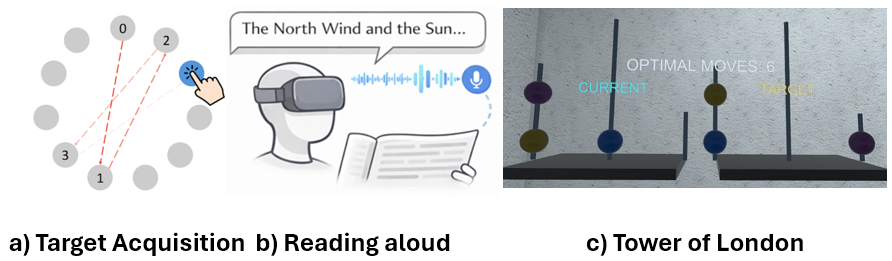
\includegraphics[width=1\linewidth]{Figure/try.png}
    \caption{The tasks used in the experiment: (a) target acquisition; (b) reading aloud; and (c) Tower of London (in-situ VR screenshot).}
    \label{fig:tasks}
\end{figure}
To investigate how acute stress affects different forms of interaction in VR, we implemented three tasks: \textit{target acquisition}, \textit{reading aloud}, and \textit{Tower of London} in a unified immersive environment (\autoref{fig:tasks}). All tasks were developed in Unity 2022.3.62f3 and deployed on a Meta Quest Pro headset using optical hand tracking (XR Hands) for controller-free interaction. We recorded physiological data with a Polar H10 chest strap, which continuously recorded heart rate and beat-to-beat (RR) intervals using Bluetooth throughout the study.
%processing details are given in ~\autoref{sec:stress-validation}.
\subsection{Tasks}
%As outlined in Section~\ref{sec:relatedwork}, 
We used MRT~\citep{wickens2008multiple} as a task-selection framework, rather than as a direct test of resource competition. The three tasks were chosen to sample different combinations of perceptual modality, processing code, response form, and central/executive demand:

\begin{itemize}
    \item \textbf{Target acquisition}: a visual-spatial task with manual response, emphasizing visuomotor coordination and fine motor control with low central planning demands.
    \item \textbf{Reading aloud}: a visual-verbal task with vocal response, emphasizing verbal encoding and speech production under controlled linguistic content.
    \item \textbf{Tower of London}: a visual-spatial task with manual response and substantial central/executive demands, emphasizing sequential planning.
\end{itemize}

Participants performed all tasks while standing, using hand tracking for direct manipulation of virtual objects. Before the experiment, they completed training trials for each task until comfortable with the interaction techniques. Task order was counterbalanced across participants using a Latin square design.

\subsubsection{Target Acquisition Task}
We implemented a target acquisition task using direct hand selection, following the methodology described in ISO 9241-411 for evaluating pointing devices. Eleven spherical targets were arranged in a circular layout 49~cm in front of the participant~\citep{li2025weight}. We instructed participants to select the highlighted targets in a displayed sequence as quickly and as accurately as possible by directly touching each sphere with their index finger. Each round comprised 11 successful selections, with a selection registered when the fingertip entered the 3~cm radius of the target.

To minimise ambiguity, the first target in each sequence was explicitly highlighted and the upcoming target was indicated in advance using a lighter shade. Upon successful selection, the system updated the highlighting to reflect the next target. A cross marker was placed at the centre of each target to indicate the intended selection point and reduce spatial uncertainty. For perceptual clarity and accessibility, all targets were rendered in blue tones, with active and upcoming targets differentiated through luminance rather than hue, avoiding reliance on red-green contrasts. An illustration of the target layout and sequential selection process is provided in Figure~\ref{fig:tasks}-(a).

\subsubsection{Target Acquisition Measures}
We recorded standard pointing performance metrics: movement time, throughput, and endpoint offset, following established evaluation methods~\citep{liu2025understanding}. Movement time (MT) was defined as the elapsed time between consecutive successful selections. Throughput (TP) was computed as a standard Fitts' law efficiency measure~\citep{mackenzie2008fitts,wobbrock2011effects}:
\[
TP = \frac{ID_e}{MT},
\]
where $ID_e$ is the effective index of difficulty. Endpoint offset was computed as the Euclidean distance between the fingertip and the target centre at the moment of selection:
\[
Offset = \sqrt{(x_f-x_c)^2 + (y_f-y_c)^2 + (z_f-z_c)^2}.
\]
Together, these metrics capture acquisition speed, the speed-accuracy trade-off, and endpoint precision.

% We additionally conducted an exploratory trajectory-based analysis of terminal pointing stability. For each successful trial, we computed the fingertip-to-target offset over the final five samples preceding selection and quantified pre-hit stability as their standard deviation:
% \[
% PreHitStability = \mathrm{SD}(offset_{t-4}, \dots, offset_t).
% \]
% Lower values indicate more stable endpoint behaviour immediately before acquisition. This measure captures fine-grained terminal variability that may not surface in aggregate outcomes. Prior motor-control work shows that mental calculation can increase postural hand tremor while leaving goal-directed kinetic tremor comparatively unchanged~\citep{budini2022mental}; we therefore treated pre-hit stability as an exploratory indicator of terminal endpoint control rather than as a direct measure of tremor.

\subsubsection{Reading Aloud Task}
We chose reading aloud rather than spontaneous speech as a task to maintain comparable linguistic content across participants and phases while still capturing stress-related changes in vocal production. Participants read excerpts from three phonetically balanced passages widely used in speech research: \textit{The North Wind and the Sun}~\citep{international1999handbook}, \textit{The Rainbow Passage}~\citep{van1972speech}, and the \textit{Grandfather Passage}~\citep{fairbanks1940voice}. To reduce passage-specific repetition and ordering effects, one passage was assigned to each experimental round using random selection without replacement, so that each participant read all three passages exactly once across the three rounds.

For experimental consistency, the passages were trimmed to approximately 110 words while preserving complete sentences, and were selected to have similar Flesch-Kincaid~\citep{kincaid1975derivation} grade levels (6.94, 7.22, and 8.16), indicating broadly comparable reading difficulty. This ensured comparable reading duration across trials while maintaining natural linguistic structure. Passages were displayed as floating text panels in the VR environment, and participants were instructed to read clearly and naturally. Audio and task timestamps were recorded for subsequent analysis.

\subsubsection{Reading Aloud Measures}
We report reading duration, mean fundamental frequency (F0), speech rate, and active speech ratio. To reduce onset hesitation and recording-start artefacts, the first 3~seconds of each recording were excluded from acoustic analysis. Reading duration served as a coarse temporal measure of task completion, while mean F0, speech rate, and active speech ratio were extracted as acoustic indicators of vocal arousal and temporal speech behaviour, following prior work in which speech-based stress and affect analysis commonly relies on prosodic and temporal features~\citep{schewski2025measuring,kappen2022acoustic}.

\subsubsection{Tower of London Task}
We implemented a VR version of the Tower of London (ToL) task~\citep{shallice1982specific} to assess executive planning and sequential problem solving. Participants were presented with an initial arrangement of coloured balls across three pegs together with a target configuration shown nearby, and were instructed to reproduce the target configuration by moving balls between pegs, subject to the constraints that only one ball could be moved at a time and that pegs had limited capacity. Participants manipulated the balls using a pinch gesture~\citep{mikkelsen2025dof}, enabling embodied interaction without controllers. The Unity application logged object states, hand-tracking events from XR Hands, move sequences, and timestamps throughout the task. Each board contained three coloured balls (8~cm in diameter) and three pegs with capacities of three, two, and one ball; adjacent peg centres were separated by 25~cm, and the current and target boards were positioned approximately 60~cm apart. 

To ensure consistent difficulty across rounds, the coloured balls and the pegs were shown in random sequence and we used ToL problems with a uniform solution depth of six moves with one rollback structure across rounds, as problem difficulty in the Tower of London is known to depend on both minimum solution length and structural characteristics of the problem~\citep{kaller2004impact}. This design avoided ceiling effects from overly simple problems and floor effects or disproportionate variability from excessively difficult ones~\citep{kaller2012assessing}. An illustration of the Tower of London task is provided in Figure~\ref{fig:tasks}-(c).

To minimise direct learning of specific configurations, we varied the spatial arrangement of balls and pegs across rounds while preserving structural difficulty, so participants encountered different instantiations rather than repeating identical layouts. This decision was also informed by pilot testing: with more repeated ToL rounds, repeated exposure substantially reduced errors over time, suggesting that learning effects could overshadow stress-related differences.

\subsubsection{Tower of London Measures}
We report first-move latency, move count, total duration, and execution time. First-move latency was defined as the interval from trial onset to the initiation of the first move, capturing the period during which participants inspected the initial and target configurations and formulated an initial plan~\citep{shallice1982specific}. Move count was the total number of moves required to reach the target configuration, with deviations from the minimum indicating less efficient planning~\citep{kaller2012assessing}. Total duration captured the time taken to complete the entire task~\citep{kaller2012assessing}, and execution time was computed as total duration minus first-move latency, allowing us to examine the time spent completing the task after movement had begun separately from initial preparation. This interval includes both object manipulation and any ongoing planning between moves~\citep{jablonska2022age}.

\subsection{Procedure}

\subsubsection{Participants}
We recruited 26 participants from the university community. After excluding two participants due to missing physiological data, the final sample consisted of 24 participants (11 female, 13 male) included in the analyses of task performance and state anxiety. Physiological recordings were available for all participants; because recording onset and signal quality varied, the number of participants contributing to each physiological analysis is reported with each result. Participants ranged in age from 20 to 31 years ($M = 24.8$, $SD = 3.0$), all reported normal or corrected-to-normal vision and no known motor impairments, and came from a range of disciplines including computer science, nursing, health, design, digital media, and psychology. The sample size is consistent with commonly adopted local standards in HCI experimental studies~\citep{caine2016local}, and recruitment with nearly equal number of male and female participants to avoid gender bias~\citep{van2009stress}. The study was approved by our institutional ethics committee, and all participants provided informed consent prior to the experiment.
\begin{figure*}[!t]
    \centering
    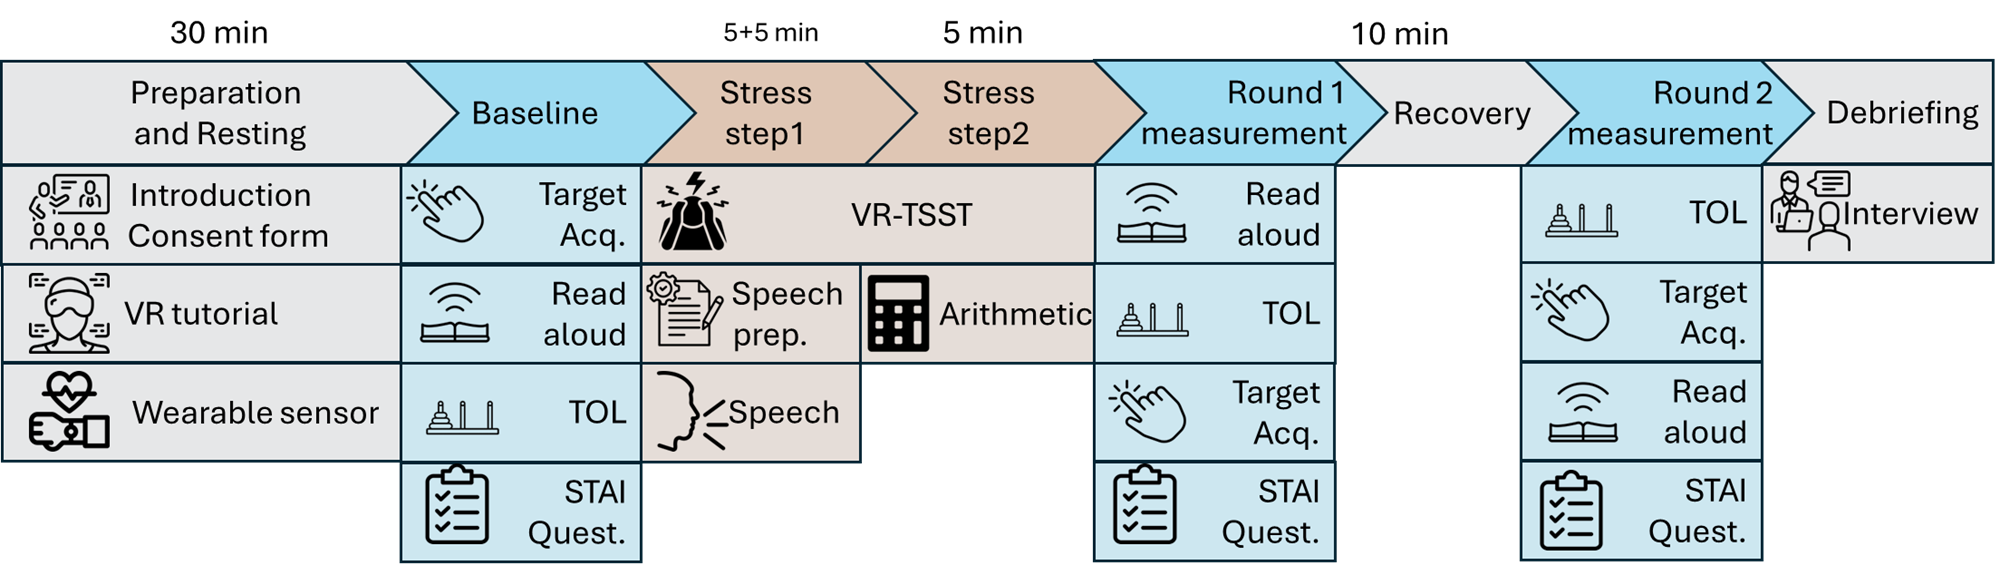
\includegraphics[width=1\textwidth]{Figure/overview.png}
    \caption{Experimental procedure. Abbreviations in the figure: Target Acq. = target acquisition; Speech prep. = speech preparation; Quest. = questionnaire. Round 1 is Post-Stress, and Round 2 is Post-Recovery Measurement.}
    \label{fig:procedure}
\end{figure*}
To induce stress, we adopted a VR adaptation of the Trier Social Stress Test (VR-TSST). The session comprised preparation and training, baseline measurement, VR-TSST stress induction, post-stress measurement, a 10-minute recovery period, and post-recovery measurement, and lasted approximately 60--70~minutes per participant. An overview is shown in~\autoref{fig:procedure}.

\subsubsection{Preparation and Training}
The experiment took place in the human-centred computing laboratory of our institution. Upon arrival, participants were fitted with a Polar H10 chest strap for physiological data collection. Before fitting the strap, the electrode areas were moistened to improve skin contact, and the strap was positioned around the participant's chest according to the manufacturer's placement guidelines. The sensor was connected via Bluetooth to the recording application, which continuously logged heart-rate estimates and RR intervals throughout the experiment. We first introduced participants to the VR system and they completed a tutorial in which they practised direct finger selection for target acquisition task and pinch gestures for the ToL task. They also rehearsed the ToL rules using a simple example problem and were given a short rest before the formal study began.


\subsubsection{Resting Period and Baseline Measurement}
We then left participants alone for 20~minutes to rest and stabilise. During this time we provided them with neutral reading material to keep them occupied without inducing anxiety, as recommended in the TSST protocol~\citep{kirschbaum1993trier}. They subsequently completed the three VR tasks and filled in the State-Trait Anxiety Inventory - State Subscale (STAI-S) questionnaire~\citep{spielberger1971state}.

\subsubsection{Stress Induction}
Participants then completed the VR-TSST and were informed that their performance would be video-recorded and reviewed by judges trained in public speaking. They were given 5~minutes to prepare a speech explaining why they would be a suitable candidate for their ideal job, followed by 5~minutes delivering the speech in front of a virtual three-member evaluation committee. Throughout preparation and delivery, the virtual committee members remained present as socially evaluative observers and provided no supportive or encouraging feedback.

Immediately after the speech, participants performed a mental arithmetic task in which they repeatedly subtracted 13 from 1022 and spoke the number sequence aloud~\citep{kirschbaum1993trier}. The same virtual committee remained present throughout, sustaining the socially evaluative atmosphere. Incorrect answers required participants to restart the calculation from the beginning. The subtraction task lasted 5~minutes.

\subsubsection{Post-Stress Measurement (Round 1)}
Immediately after stress induction, participants completed the first post-stress measurement round, again performing the three VR tasks and filling in the STAI questionnaire. Task order differed from the baseline stage to reduce learning effects. This round began immediately following the completion of the VR-TSST and was completed immediately after the STAI-S for this round, ensuring that all post-stress behavioral measurements were captured.

\subsubsection{Recovery and Post-Recovery Measurement (Round 2)}
Following the post-stress measurement round, participants were given a 10~minute recovery period. To improve comfort and reduce headset fatigue, they were asked to remove the headset and rest quietly. After the recovery period, participants completed the second measurement round and filled in the STAI questionnaire. This round is referred to as Post-Recovery. The measurement was conducted after the completion of Round 1 and before the subsequent task round began.

\subsubsection{Participant Debriefing}
Finally, we debriefed participants about the study, explained that experiencing stress during the experiment was expected, and clarified that the tasks were intentionally demanding and did not reflect participants' aptitude or ability. We also informed them that their performance had not been evaluated by a real judging panel. We then conducted a short semi-structured interview, asking participants to report their subjective perception of the experiment and the effect of stress on their performance.

\subsection{Stress Measures and Analysis Windows}
\label{sec:stress-validation}

We assessed state anxiety using the state scale of the State-Trait Anxiety Inventory (STAI-S) at the end of each measurement round~\citep{spielberger1971state}. Heart rate (HR) and RR intervals were recorded continuously using a Polar H10 chest strap. Heart rate variability (HRV) measures served as the primary physiological measures, with HR as a secondary measure. We analysed the physiological data in two ways: as mean values within three protocol windows and three task rounds, and as a continuous time series across the whole session.

The protocol windows included the Baseline, Induction, and Recovery windows. The Baseline window extended from the start of the Polar recording to the onset of the first task round. The Induction window covered the whole VR-TSST, from the start of speech preparation to the end of mental arithmetic. The Recovery window extended from submission of the Post-Stress STAI-S to the onset of the Post-Recovery round, while participants rested without the headset. Each task round extended from the onset of its first task to submission of its STAI-S, encompassing the three task probes and the questionnaire completed in VR. The median task-round duration was 3.4~min.

 RR intervals were exported in units of 1/1024~s and converted to milliseconds. Because one Bluetooth notification could contain several RR intervals, beat times were reconstructed by accumulating the intervals within each notification. Intervals outside 250-2500~ms were treated as invalid. One or two consecutive intervals that deviated from the median of the ten surrounding intervals by more than $\max(150~\mathrm{ms}, 6\times\mathrm{MAD})$ and by a ratio below 0.65 or above 1.5 were replaced by linear interpolation when the neighbouring intervals agreed within 20\%, and were otherwise excluded. 
 We computed the natural logarithm of the root mean square of successive differences (lnRMSSD) in non-overlapping 60-s windows and the natural logarithm of high-frequency power (log HF-HRV; 0.15--0.40~Hz) in non-overlapping 128-s windows, using a Hann-windowed periodogram of the RR series resampled at 4~Hz~\citep{shaffer2017overview}. A window was accepted when valid beats covered at least 80\% of its duration and no more than 5\% of its intervals had been edited, and accepted window values were averaged within each protocol window. Because each task round lasted only a few minutes, lnRMSSD and log HF-HRV were computed over the whole round. Mean HR was computed from the heart-rate values reported by the device.

To characterise the time course across the whole session, we computed lnRMSSD and HR in 60-s windows and log HF-HRV in 128-s windows, advanced in 30-s steps from five minutes before the first task round to the end of the last round. For visualisation, each participant's phase boundaries were linearly aligned to the median phase durations, and values were expressed as changes from the participant's Baseline window.

\subsection{Statistical Analysis}

Stress reactivity and recovery describe complementary processes following a stressor~\citep{linden1997physiological,chida2008chronic}. We refer to the change from Baseline to Post-Stress (or Induction) as reactivity and the change from Post-Stress (or Induction) to Post-Recovery (or Recovery) as recovery.

Completion-time measures (target-acquisition movement time, reading duration, and Tower of London first-move latency, execution time, and total duration) were strictly positive and right-skewed, with variability increasing with the mean. These measures were analysed with generalised linear mixed-effects models (GLMMs) with a Gamma distribution and log link~\citep{lo2015transform}, including phase as a fixed effect and a random intercept for each participant; the effect of phase was tested with a Wald $\chi^2$ test. All other measures (STAI-S, throughput, endpoint offset, mean $F_0$, speech rate, active speech ratio, Tower of London move count, and the physiological measures lnRMSSD, log HF-HRV, and HR, separately for the protocol windows and the task rounds) were analysed using one-way repeated-measures ANOVAs with phase as the within-participant factor, reporting Greenhouse-Geisser-corrected $p$ values. For both model types, pairwise differences between the three phases were Tukey-adjusted, controlling the family-wise error rate across the three comparisons within each measure; for the ANOVAs, Tukey HSD tests were based on the repeated-measures error term. Physiological ANOVAs included the participants with valid values in all three phases of the respective analysis.
% STAI-S, task measures, and the physiological measures (lnRMSSD, log HF-HRV, and HR, separately for the protocol windows and the task rounds) were analysed using one-way repeated-measures ANOVAs with phase as the within-participant factor, reporting Greenhouse--Geisser-corrected $p$ values. Pairwise differences between the three phases were assessed using Tukey HSD tests based on the repeated-measures error term, which control the family-wise error rate across the three comparisons within each measure. Physiological ANOVAs included the participants with valid values in all three phases of the respective analysis.


Within-phase trends were examined with a piecewise linear mixed-effects model fitted to non-overlapping windows (60~s for lnRMSSD and HR; 128~s for log HF-HRV). The model included a separate level for each phase and a separate linear slope for each phase lasting at least five minutes (the final five minutes of the Baseline window, Preparation, Speech, Arithmetic, and Recovery), with a random intercept for each participant. Slopes were tested against zero with Holm correction within each measure.

We report partial eta squared ($\eta_p^2$) for ANOVA effects and, for each pairwise comparison, the mean difference with its 95\% confidence interval and Cohen's $d_z$ (later minus earlier phase). For the Gamma GLMMs, pairwise effects are reported as ratios of model-estimated means (later/earlier) with Tukey-adjusted simultaneous 95\% confidence intervals.

Although several difference scores deviated from normality (Shapiro-Wilk $p<.05$), repeated-measures ANOVA is robust to such violations when sphericity holds~\citep{blanca2023datos}. All physiological data processing and statistical analyses were conducted in Python using custom scripts with pandas, NumPy, SciPy, statsmodels, and Matplotlib.

% We validated stress occurrence using participants' self-reported anxiety and physiological responses. We measured self-reported anxiety with the state scale of the State-Trait Anxiety Inventory – State scale (STAI-S) after each round~\citep{spielberger1971state}. We recorded physiological responses  with a Polar H10 chest strap. To calculate high-frequency heart rate variability (HF HRV), a frequency-domain measure of heart rate variability (HRV),we extracted heart rate and inter-beat interval (IBI) estimates derived from the RR intervals. Following prior work~\citep{sarsenbayeva2019measuring}, We ordered IBI samples by timestamp, interpolated them to a uniformly sampled 4~Hz time series, and analysed using an Fast Fourier Transform (FFT)-based sliding-window procedure. For each 512-sample window, we computed the frequency spectrum and summed spectral magnitude within the high-frequency band (HF HRV: 0.15--0.40~Hz). HF HRV values were averaged within each physiological analysis window and log-transformed before statistical analysis. In addition to HF HRV, we computed mean heart rate (HR) and the standard deviation of normal-to-normal intervals (SDNN) as indicators of cardiovascular arousal. Although the root mean square of successive differences between normal heartbeats (RMSSD) is often used as an index of parasympathetic activity, the VR-TSST in our study involved continuous speech and aloud arithmetic tasks, which may directly affect short-term beat-to-beat variability. We therefore use SDNN as the primary time-domain HRV measure and treat RMSSD as a complementary measure~\citep{shaffer2017overview}. All physiological data processing and statistical analyses were conducted in Python using custom scripts with pandas, NumPy, SciPy, and Matplotlib.





\section{Results}

\subsection{Stress Validation}

We report stress-validation results for the protocol windows (Baseline, Induction, Recovery) and the task rounds (Baseline, Post-Stress, Post-Recovery). STAI-S analyses included $n=24$; the number of participants in each physiological analysis is reported with each result. STAI-S is reported as scale scores, HR in beats per minute (bpm), and lnRMSSD and log HF-HRV as geometric means (ms and ms$^2$) with percentage changes. Pairwise $p$ values are Tukey-adjusted, and confidence intervals are 95\% intervals of the mean difference.

\subsubsection{Stress Induction}
STAI-S scores (\autoref{fig:stai}) showed a significant effect of phase, $F(2,46)=25.77$, $p<.001$, $\eta_p^2=.528$. Self-reported anxiety rose from Baseline ($M=32.38$, $SD=7.83$) to Post-Stress ($M=47.58$, $SD=10.29$), an increase of 15.21 points, 95\% CI $[10.52, 19.89]$, $d_z=1.37$, $p<.001$.

In the protocol windows, lnRMSSD varied across phases ($n=23$), $F(2,44)=19.96$, $p<.001$, $\eta_p^2=.476$. RMSSD was 22.8\% lower during Induction (geometric mean 21.0~ms) than in the Baseline window (27.1~ms), 95\% CI $[-32.2\%, -12.0\%]$, $d_z=-0.86$, $p<.001$. log HF-HRV also varied across phases ($n=22$), $F(2,42)=9.63$, $p<.001$, $\eta_p^2=.314$, but did not differ between the Baseline window (156.4~ms$^2$) and Induction (164.9~ms$^2$; $+5.4\%$, 95\% CI $[-19.1\%, +37.3\%]$, $d_z=0.09$, $p=.914$). HR varied across phases ($n=23$), $F(2,44)=31.58$, $p<.001$, $\eta_p^2=.589$, increasing from the Baseline window ($M=87.29$~bpm, $SD=9.34$) to Induction ($M=92.53$, $SD=10.74$) by 5.24~bpm, 95\% CI $[3.19, 7.29]$, $d_z=1.11$, $p<.001$.

Comparison with the Baseline round, which was also performed in VR, qualified these differences. lnRMSSD ($-0.9\%$, $p=.789$) and log HF-HRV ($+12.4\%$, $p=.209$) did not differ between Induction and the Baseline round, whereas HR was 1.63~bpm higher during Induction ($p=.025$; paired $t$ tests), most clearly in the first minute of the speech ($+7.01$~bpm, $p<.001$). The time course (\autoref{fig:timeseries}) showed that HR tended to rise during speech preparation (0.69~bpm/min, 95\% CI $[0.10, 1.27]$, Holm-adjusted $p=.089$), peaked at the onset of the speech, and declined during the speech by 1.19~bpm/min (95\% CI $[-1.78, -0.60]$, Holm-adjusted $p<.001$). No within-phase trend was significant for lnRMSSD or log HF-HRV (all Holm-adjusted $p \geq .61$); these measures shifted between phases rather than changing gradually within them.

Across the three task rounds, lnRMSSD ($n=23$), $F(2,44)=2.52$, $p=.094$, $\eta_p^2=.103$, and HR ($n=24$), $F(2,46)=3.01$, $p=.071$, $\eta_p^2=.116$, did not differ significantly. log HF-HRV ($n=19$) varied across rounds, $F(2,36)=7.33$, $p=.003$, $\eta_p^2=.289$; it did not differ between the Baseline and Post-Stress rounds ($-7.2\%$, $p=.755$) but was higher in the Post-Recovery round than in the Post-Stress round ($+46.0\%$, $p=.003$) and the Baseline round ($+35.5\%$, $p=.017$). For all three measures, the Post-Stress round did not differ from the Baseline round (all Tukey-adjusted $p \geq .75$, $|d_z| \leq 0.18$), although STAI-S scores collected at the end of the Post-Stress round remained elevated. Together, these results show that the VR-TSST elevated subjective anxiety and produced a heart-rate response that exceeded the level of VR task performance, most clearly at the onset of the speech, whereas lower HRV during Induction than in the Baseline window also reflected the context of acting in VR.

\subsubsection{Recovery}
STAI-S scores declined from Post-Stress to Post-Recovery ($M=35.25$, $SD=11.58$), a decrease of 12.33 points, 95\% CI $[-16.77, -7.89]$, $d_z=-1.17$, $p<.001$, and no longer differed from Baseline ($p=.415$).

In the protocol windows, HR decreased from Induction to Recovery ($M=83.79$~bpm, $SD=8.44$) by 8.74~bpm, 95\% CI $[-11.31, -6.18]$, $d_z=-1.47$, $p<.001$, and was lower than in the Baseline window ($-3.50$~bpm, 95\% CI $[-5.74, -1.26]$, $p=.008$). RMSSD increased from Induction to Recovery (29.7~ms) by 41.6\%, 95\% CI $[+26.5\%, +58.6\%]$, $d_z=1.33$, $p<.001$, and did not differ from the Baseline window ($+9.4\%$, $p=.272$). log HF-HRV increased from Induction to Recovery (262.3~ms$^2$) by 59.1\%, 95\% CI $[+22.9\%, +105.9\%]$, $d_z=0.80$, $p=.002$, and exceeded its Baseline-window value ($+67.7\%$, $p<.001$). Because participants removed the headset and rested quietly during Recovery, differences from the Baseline window may also reflect this change in activity.

Overall, STAI-S no longer differed from Baseline after recovery, and HR and HRV changed in the opposite direction to the induction response. \autoref{tab:all-change-summary} summarises the reactivity and recovery changes.

% \subsection{Validation of Stress Occurrence}

% We first examined whether the VR-TSST successfully induced stress. We analysed STAI-S, mean HR, SDNN, and log-transformed HF-HRV across phases. 

% STAI state scores showed a statistically significant effect of phase, $F(2,46)=25.77, p<.001$. Participants reported significantly higher anxiety after stress induction (Baseline: $M=32.38$, $SD=7.83$; Post-Stress: $M=47.58$, $SD=10.29$; Baseline vs.\ Post-Stress: $p<.001$), followed by a significant decrease during Recovery (Recovery: $M=35.25$, $SD=11.58$; Post-Stress vs.\ Recovery: $p<.001$). No significant difference was observed between Baseline and Recovery ($p=.231$). These result shows in ~\autoref{fig:stai} indicate that the protocol successfully increased subjective anxiety during the stress-induction phase.


% Mean HR shows in ~\autoref{fig:hr} also showed a statistically significant effect of phase, $F(2,46)=31.12, p<.001$. Mean HR increased from Baseline ($M=88.10$ bpm, $SD=9.03$) to Stress Induction ($M=92.13$ bpm, $SD=10.62$; Baseline vs.\ Stress Induction: $p<.001$), and significantly decreased during Post-stress Recovery ($M=83.85$ bpm, $SD=8.41$; Stress Induction vs.\ Post-stress Recovery: $p<.001$). Baseline and Recovery also differed significantly ($p<.001$), indicating a substantial reduction in physiological arousal after the stress period.

% We further examined HRV using SDNN. SDNN in ~\autoref{fig:sdnn} showed a significant phase effect, $F(2,42)=8.35, p<.001$. SDNN decreased from Baseline ($M=72.58$ ms, $SD=34.27$) to Stress Induction ($M=57.56$ ms, $SD=21.75$; Baseline vs.\ Stress Induction: $p=.006$), and increased during Post-stress Recovery ($M=73.50$ ms, $SD=22.59$; Stress Induction vs.\ Post-stress Recovery: $p=.001$). Baseline and Recovery did not significantly differ ($p=.819$). Since lower SDNN values indicate reduced HRV and elevated physiological arousal, these results provide further evidence that the stress induction successfully altered participants' physiological state.


% For comparison with prior stress-interaction work, we also examined frequency-domain HF-HRV~\ref{fig:hrv_fft}. The repeated-measures ANOVA on log-transformed HF-HRV showed a statistically significant effect of phase, $F(2,42)=3.28, p=.047$. Although the decrease from Baseline to Stress Induction did not reach significance (Baseline: $M=10.57$, $SD=0.89$; Stress Induction: $M=10.40$, $SD=0.75$; $p=.122$), HF-HRV significantly increased from Stress Induction to Post-stress Recovery (Recovery: $M=10.64$, $SD=0.76$; $p=.017$). 
% Together, the STAI, HR, and HRV results indicate that the stress-induction protocol successfully increased both subjective anxiety and physiological arousal. For ease of comparison across validation measures, ~\autoref{tab:validation-change} summarises the direction and magnitude of percentage changes between adjacent phases.
\begin{figure}[t]
\centering
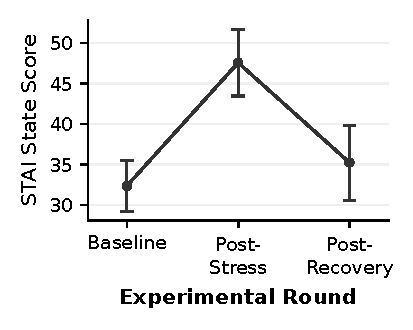
\includegraphics[width=0.7\columnwidth]{Figure/stress_stai.pdf}
\caption{State anxiety (STAI-S) at the end of each measurement round ($n=24$). Error bars show 95\% confidence intervals.}
\label{fig:stai}
\end{figure}

\begin{figure*}[t]
\centering
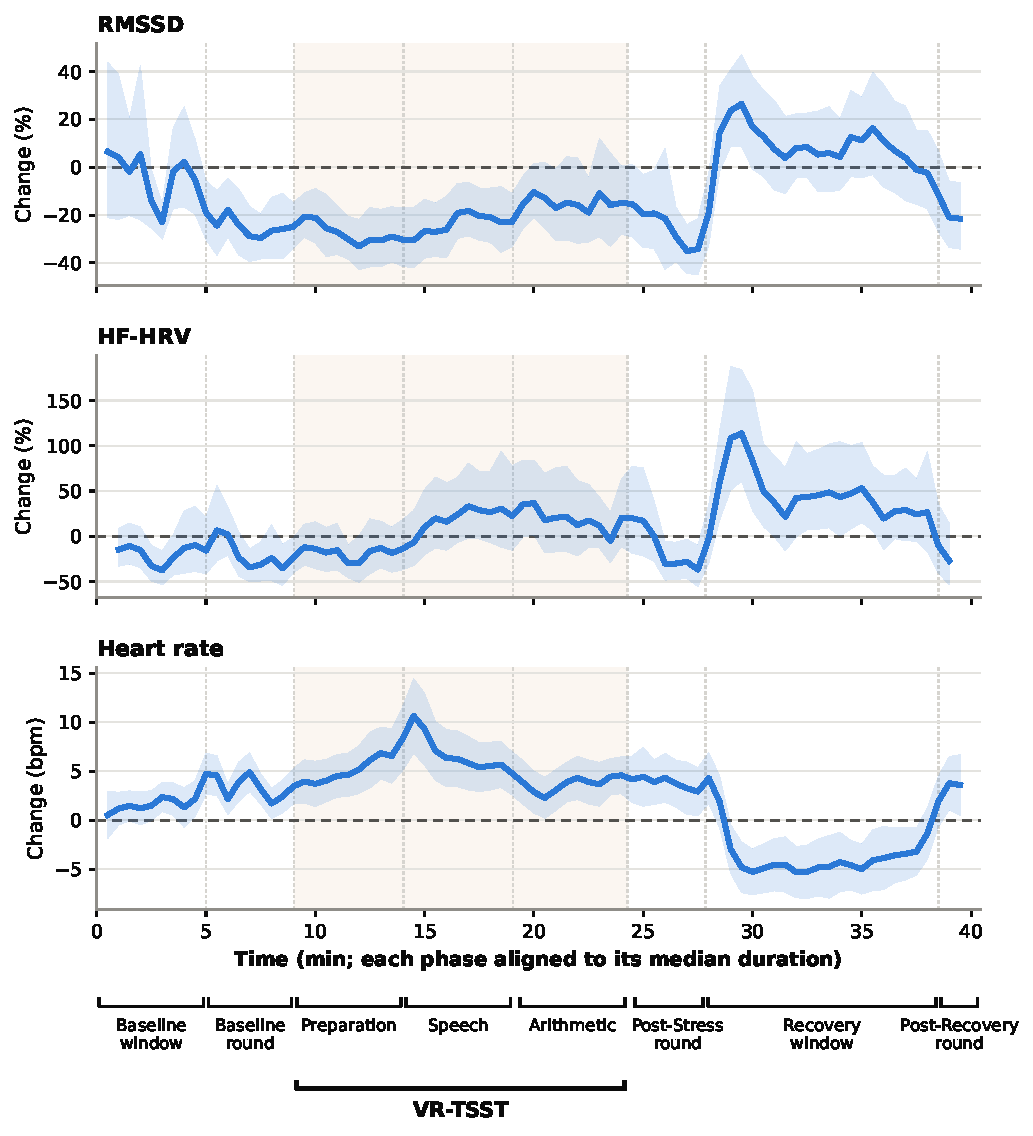
\includegraphics[width=0.92\textwidth]{Figure/stress_timeseries.pdf}
\caption{Physiological time course across the session, shown as the mean change from each participant's Baseline window ($\pm$ 95\% confidence interval). RMSSD and heart rate were computed in 60-s windows and HF-HRV in 128-s windows, advanced in 30-s steps; each participant's phases were linearly aligned to the median phase durations. The timeline above the panels marks the protocol phases.}
\label{fig:timeseries}
\end{figure*}


\subsection{Target Acquisition Task}
We next examined target acquisition task performance using mean movement time, Fitts' throughput, and endpoint offset (\autoref{tab:phase-comparisons}). Phase had no significant effect on movement time (Gamma GLMM, $\chi^2(2)=0.04$, $p=.981$), throughput ($F(2,46)=0.09$, $p=.905$), or offset ($F(2,46)=0.35$, $p=.683$), and Tukey-adjusted pairwise comparisons revealed no significant differences between any pair of phases (all $p \geq .71$, $|d_z| \leq 0.20$). Movement time differed by less than 1\% between any two phases (model-estimated ratios 0.996--1.008), and the effects on throughput and offset were negligible ($\eta_p^2=.004$ and $.015$). Between Baseline and Post-Stress, movement time differed by $+17.67$~ms, 95\% CI $[-93.93, +129.26]$; throughput by $-0.02$~bit/s, 95\% CI $[-0.36, +0.33]$; and offset by $+0.05$~cm, 95\% CI $[-0.05, +0.15]$.

% Beyond these predefined metrics, we conducted an exploratory analysis of terminal pointing stability, defined as the standard deviation of the finger-to-target-centre offset across the final five samples before successful selection (lower values indicate more stable terminal movements). Mean pre-hit variability (~\autoref{fig:tara}-a) decreased from Baseline ($M=0.341$) to Post-Stress ($M=0.275$) and rose again at Post-Recovery ($M=0.323$). The overall phase effect did not reach significance ($p=.127$).Uncorrected contrasts indicated a decrease from Baseline to Post-Stress ($p=.025$) and an increase from Post-Stress to Post-Recovery ($p=.049$); neither would survive correction for two comparisons, so this pattern should be treated as exploratory. It tentatively suggests that terminal hand movements became more stable during the stress phase, even though conventional endpoint measures showed no change. ~\autoref{tab:all-change-summary} summarises the phase-wise changes in the predefined target acquisition measures and the exploratory pre-hit variability measure.
% , but pairwise comparisons indicated a significant decrease from Baseline to Post-Stress ($p=.025$) and a significant increase from Post-Stress to Post-Recovery ($p=.049$). This suggests that terminal hand movements may have become more stable during the stress phase, even though conventional endpoint measures showed no significant change. ~\autoref{tab:all-change-summary} summarises the phase-wise direction and magnitude of change across target acquisition measures,\autoref{tab:all-change-summary} summarises the observed phase-wise changes in the predefined target acquisition measures and the exploratory pre-hit variability measure.

% \subsubsection{Target Acquisition}

% We then investigated the effect of stress on target acquisition performance using mean target acquisition time, Fitts' throughput, and endpoint offset size. A one-way repeated-measures ANOVA showed no statistically significant effect of phase on target acquisition time ($F(2,46)=0.10, p=.907$), throughput ($F(2,46)=0.09, p=.912$), or offset size ($F(2,46)=0.35, p=.708$). Pairwise comparisons also revealed no statistically significant differences between Baseline and Post-Stress or between Post-Stress and Recovery for any of these measures (all $p>.05$). These results indicate that stress induction did not significantly affect target acquisition speed, throughput, or endpoint accuracy in our XR task.

% Beyond the predefined target acquisition metrics, we also conducted an exploratory analysis of terminal pointing stability using the standard deviation of the finger-to-target-center offset during the final five pre-hit samples before successful selection. Lower values indicate more stable hand movements immediately before target acquisition. Mean pre-hit offset variability in ~\autoref{fig:std} decreased from Baseline ($M=0.341$) to Post-Stress ($M=0.275$), and then increased again during Recovery ($M=0.323$). Although the overall phase effect did not reach significance ($p=.127$), pairwise comparisons indicated a significant decrease from Baseline to Post-Stress ($p=.025$) and a significant increase from Post-Stress to Recovery ($p=.049$). This suggests that terminal hand movements may have become more stable during the stress phase, even though conventional endpoint offset measures did not show significant changes. ~\autoref{tab:ta-change} provides a compact summary of the phase-wise direction and magnitude of change across target acquisition measures, highlighting the contrast between stable predefined outcomes and the exploratory terminal stability metric.




% \begin{figure}[t]
% \centering
% \begin{subfigure}[t]{0.48\columnwidth}
%     \centering
%     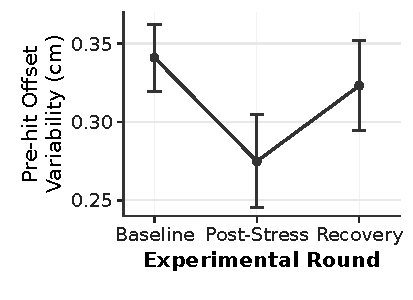
\includegraphics[width=\linewidth]{Figure/prehit_stability.pdf}
%     \caption{Exploratory terminal pointing stability}
%     \label{fig:prehit-stability}
% \end{subfigure}\hfill
% \begin{subfigure}[t]{0.48\columnwidth}
%     \centering
%     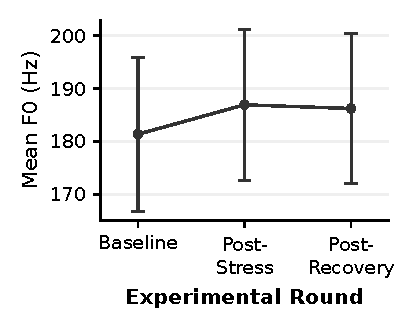
\includegraphics[width=\linewidth]{Figure/reading_mean_f0.pdf}
%     \caption{Reading aloud mean F0}
%     \label{fig:reading-f0}
% \end{subfigure}

% \caption{Stress-related changes in target acquisition task and reading aloud task. Error bars show 95\% confidence intervals.}
% \label{fig:tara}
% \end{figure}
\begin{figure}[t]
\centering
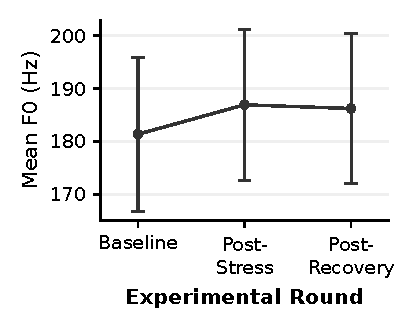
\includegraphics[width=0.6\columnwidth]{Figure/reading_mean_f0.pdf}
\caption{Mean $F_0$ during reading aloud across phases. Error bars show 95\% confidence intervals.}
\label{fig:tara}
\end{figure}
\subsection{Reading Aloud Task}
% We then examined reading aloud performance using reading duration, mean fundamental frequency (F0), speech rate, and active speech ratio. A one-way repeated-measures ANOVA showed a significant effect of phase on mean F0 ($F(2,46)=4.26, p=.020$): F0 was higher in Post-Stress ($M=186.91$~Hz, $SD=35.62$) than in Baseline ($M=181.35$~Hz, $SD=36.36$; $p=.020$), but did not differ significantly between Post-Stress and Post-Recovery ($M=186.20$~Hz, $SD=35.38$; $p=.689$). Reading duration, speech rate, and active speech ratio did not show significant effects of phase (all $p>.05$). Mean values are visualised in ~\autoref{fig:tara}-b, and ~\autoref{tab:all-change-summary} summarises the phase-wise percentage changes across vocal measures. The effect on mean F0 was moderate, $\eta_p^2=.156$; F0 rose by 5.55~Hz from Baseline to Post-Stress, 95\% CI $[+0.96, +10.15]$. The remaining vocal measures showed negligible effects: reading duration $F(2,46)=0.27$, $p=.765$, $\eta_p^2=.012$; speech rate $F(2,46)=0.85$, $p=.432$, $\eta_p^2=.036$; active speech ratio $F(2,46)=0.91$, $p=.409$, $\eta_p^2=.038$.
We then examined reading aloud performance using reading duration, mean fundamental frequency (F0), speech rate, and active speech ratio. A one-way repeated-measures ANOVA showed a significant effect of phase on mean F0 ($F(2,46)=4.26, p=.023$): F0 was higher in Post-Stress ($M=186.91$~Hz, $SD=35.62$) than in Baseline ($M=181.35$~Hz, $SD=36.36$; $p=.027$, $d_z=0.51$), with no significant difference between Post-Stress and Post-Recovery ($M=186.20$~Hz, $SD=35.38$; $p=.938$) or between Baseline and Post-Recovery ($p=.060$). Reading duration, speech rate, and active speech ratio did not show significant effects of phase (all $p>.05$) or pairwise differences (all Tukey $p \geq .42$). Mean values are visualised in ~\autoref{fig:tara}, and ~\autoref{tab:all-change-summary} summarises the phase-wise percentage changes across vocal measures. The effect on mean F0 was moderate, $\eta_p^2=.156$; F0 rose by 5.55~Hz from Baseline to Post-Stress, 95\% CI $[+0.96, +10.15]$. The remaining vocal measures showed negligible effects: reading duration (Gamma GLMM) $\chi^2(2)=0.53$, $p=.769$; speech rate $F(2,46)=0.85$, $p=.426$, $\eta_p^2=.036$; active speech ratio $F(2,46)=0.91$, $p=.407$, $\eta_p^2=.038$.
% \subsubsection{Reading Aloud}

% We next examined the effect of stress on read-aloud performance using reading duration, mean fundamental frequency (F0), speech rate, and active speech ratio. The first 3 seconds of each recording were excluded to reduce onset hesitation and recording-start artifacts. A one-way repeated-measures ANOVA showed a statistically significant effect of phase on mean F0 ($F(2,46)=4.26, p=.020$). Pairwise comparisons indicated that mean F0 was significantly higher in the Post-Stress phase ($M=186.91$ Hz, $SD=35.62$) than in Baseline ($M=181.35$ Hz, $SD=36.36$; $p=.020$). However, no statistically significant difference was observed between Post-Stress and Recovery (Recovery: $M=186.20$ Hz, $SD=35.38$; $p=.689$). In contrast, reading duration, speech rate, and active speech ratio did not show statistically significant effects of phase (all $p>.05$). These results suggest that stress induction altered participants' vocal arousal, while leaving coarse speech timing measures relatively stable. The mean values for read-aloud measures are visualised in ~\autoref{fig:ra}, while ~\autoref{tab:ra-change} summarises the phase-wise percentage changes to facilitate comparison across vocal measures.

\subsection{Tower of London Task}
% Finally, we examined ToL task performance using first-move latency, move count, total duration, and execution time.
% The repeated-measures ANOVA on total duration were not significant ($F(2,46)=2.50, p=.093$). However, pairwise comparisons showed that total duration(~\autoref{fig:tol}-a) was significantly shorter in Post-Stress ($M=36.22$~s, $SD=16.12$) than in Baseline ($M=51.54$~s, $SD=35.86$; $p=.009$), with no significant difference between Post-Stress and Post-Recovery ($M=43.84$~s, $SD=26.00$; $p=.179$). A similar pattern emerged for execution time (~\autoref{fig:tol}-b): the omnibus test was not significant ($F(2,46)=2.26, p=.116$), but execution time was significantly shorter in Post-Stress ($M=20.51$~s, $SD=13.76$) than in Baseline ($M=34.02$~s, $SD=29.02$; $p=.007$), with no significant difference between Post-Stress and Post-Recovery ($p=.348$). First-move latency and move count showed no significant phase effects (all $p>.05$). Both timing effects were small to moderate in size ($\eta_p^2=.098$ for total duration and $.089$ for execution time). Total duration was 15.32~s shorter in Post-Stress than Baseline, 95\% CI $[-26.51, -4.13]$, and execution time 13.52~s shorter, 95\% CI $[-23.00, -4.04]$. The planning measures showed negligible effects: first-move latency $F(2,46)=0.27$, $p=.767$, $\eta_p^2=.011$; move count $F(2,46)=0.80$, $p=.456$, $\eta_p^2=.034$.
Gamma GLMMs showed a significant effect of phase on execution time, $\chi^2(2)=8.15$, $p=.017$, and total duration, $\chi^2(2)=7.63$, $p=.022$, but not on first-move latency, $\chi^2(2)=1.00$, $p=.606$. Move count did not vary across phases ($F(2,46)=0.80$, $p=.451$, $\eta_p^2=.034$). Execution time was 36.0\% shorter in Post-Stress than in Baseline (ratio $=0.64$, 95\% CI $[0.44, 0.92]$, $p=.012$; $M=20.51$~s, $SD=13.76$ vs.\ $M=34.02$~s, $SD=29.02$; $d_z=-0.60$), and 19 of 24 participants were faster. Total duration was 24.9\% shorter (ratio $=0.75$, 95\% CI $[0.58, 0.97]$, $p=.021$; $M=36.22$~s vs.\ $51.54$~s; $d_z=-0.58$) (\autoref{fig:tol}). Post-Recovery did not differ from Baseline or Post-Stress on either measure (all $p > .13$). These reductions depended on the model and on individual participants: in linear mixed models on log-transformed times, they were smaller and not significant (execution time $-31.7\%$, $p=.091$; total duration $-20.9\%$, $p=.130$). The execution-time difference remained significant when any single participant was excluded (all $p \leq .037$), whereas the total-duration difference did not when either of two participants with long Baseline times was excluded.

Thus, planning measures did not change after stress induction, whereas execution time was shorter in the Post-Stress round.
% \subsubsection{Tower of London}

% We then investigated the effect of stress on Tower of London (ToL) performance using first-move latency, move count, total duration and execution time. Execution time was computed as total task duration minus first-move latency, capturing the time spent executing moves after the initial planning period.

% A one-way repeated-measures ANOVA did not show a statistically significant effect of phase on total duration ($F(2,46)=2.28, p=.114$)~\ref{fig:tol_dur}. However, pairwise comparisons indicated that total duration was significantly shorter in the Post-Stress phase ($M=36.22$ s, $SD=16.12$) than in Baseline ($M=50.87$ s, $SD=36.30$; $p=.013$). No statistically significant difference was observed between Post-Stress and Recovery (Recovery: $M=44.51$ s, $SD=25.58$; $p=.147$).


\begin{figure}[t]
\centering
\begin{minipage}[t]{0.48\textwidth}
    \centering
    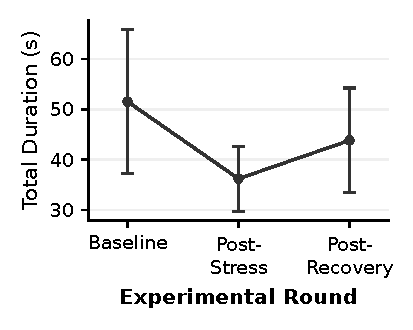
\includegraphics[width=\linewidth]{Figure/tol_total_duration.pdf}\\
    {\small (a) Total duration}
\end{minipage}\hfill
\begin{minipage}[t]{0.48\textwidth}
    \centering
    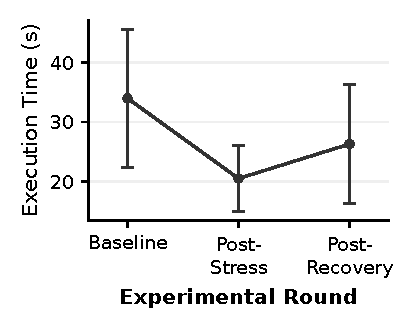
\includegraphics[width=\linewidth]{Figure/tol_execution_time.pdf}\\
    {\small (b) Execution time}
\end{minipage}
\caption{Tower of London timing measures across experimental phases: (a) total duration and (b) execution time. Execution time and total duration were shorter in Post-Stress than in Baseline (Gamma GLMM, Tukey-adjusted $p=.012$ and $p=.021$); no other pairwise difference was significant. Error bars show 95\% confidence intervals.}
\label{fig:tol}
\end{figure}
% Similarly, a one-way repeated-measures ANOVA did not show a statistically significant effect of phase on execution time ($F(2,46)=1.98, p=.149$)~\ref{fig:tol_exe}. Nevertheless, pairwise comparisons showed that execution time was significantly shorter in the Post-Stress phase ($M=20.51$ s, $SD=13.76$) than in Baseline ($M=33.29$ s, $SD=29.38$; $p=.010$). No statistically significant difference was found between Post-Stress and Recovery ($p=.295$).

% In contrast, first-move latency and move count did not show statistically significant effects of phase (all $p>.05$). Taken together, these results indicate that stress induction did not broadly improve ToL planning performance, but was associated with faster task execution following stress induction. This reduction in execution time should be interpreted cautiously, as it may reflect faster or more urgent task execution rather than a broad enhancement of planning ability. ~\autoref{tab:tol-change} summarises the direction and relative magnitude of phase-wise changes across Tower of London measures, showing that the clearest shifts were observed in total duration and execution time rather than in planning-specific measures.
\begin{table*}[t]
\centering
\caption{Three-phase comparisons of state anxiety and task measures ($n=24$).}
\label{tab:phase-comparisons}
\small
\setlength{\tabcolsep}{7pt}
\renewcommand{\arraystretch}{1.22}
\resizebox{\textwidth}{!}{%
\begin{tabular}{@{}l r r r r r r r@{}}
\toprule
 & Overall & \multicolumn{2}{c}{1--2} & \multicolumn{2}{c}{2--3} & \multicolumn{2}{c}{1--3} \\
\cmidrule(lr){3-4}\cmidrule(lr){5-6}\cmidrule(lr){7-8}
Measure & $p$
 & $p_{\mathrm{Tukey}}$ & $d_z$
 & $p_{\mathrm{Tukey}}$ & $d_z$
 & $p_{\mathrm{Tukey}}$ & $d_z$ \\
\midrule
STAI-S & $\mathbf{<.001}$ & $\mathbf{<.001}$ & $+1.37$ & $\mathbf{<.001}$ & $-1.17$ & $.415$ & $+0.25$ \\
\midrule
Movement time$^{\dagger}$ & $.981$ & $.979$ & $+0.07$ & $.995$ & $-0.08$ & $.994$ & $0.00$ \\
Throughput & $.905$ & $.996$ & $-0.02$ & $.945$ & $-0.06$ & $.913$ & $-0.08$ \\
Endpoint offset & $.683$ & $.713$ & $+0.20$ & $.988$ & $-0.03$ & $.801$ & $+0.13$ \\
\midrule
Mean $F_0$ & $\mathbf{.023}$ & $\mathbf{.027}$ & $+0.51$ & $.938$ & $-0.08$ & $.060$ & $+0.45$ \\
Reading duration$^{\dagger}$ & $.769$ & $.998$ & $+0.09$ & $.820$ & $-0.14$ & $.791$ & $-0.06$ \\
Speech rate & $.426$ & $.942$ & $+0.07$ & $.424$ & $-0.30$ & $.624$ & $-0.17$ \\
Active speech ratio & $.407$ & $.985$ & $-0.03$ & $.532$ & $-0.24$ & $.434$ & $-0.24$ \\
\midrule
ToL first-move latency$^{\dagger}$ & $.606$ & $.759$ & $-0.14$ & $.598$ & $+0.15$ & $.964$ & $0.00$ \\
ToL move count & $.451$ & $.654$ & $-0.20$ & $.445$ & $+0.25$ & $.937$ & $+0.06$ \\
ToL execution time$^{\dagger}$ & $\mathbf{.017}$ & $\mathbf{.012}$ & $-0.60$ & $.319$ & $+0.20$ & $.384$ & $-0.20$ \\
ToL total duration$^{\dagger}$ & $\mathbf{.022}$ & $\mathbf{.021}$ & $-0.58$ & $.138$ & $+0.28$ & $.739$ & $-0.17$ \\
\bottomrule
\end{tabular}}

\medskip
\begin{minipage}{0.98\textwidth}
\footnotesize
\textit{Notes.} 1 = Baseline; 2 = Post-Stress; 3 = Post-Recovery.
$^{\dagger}$Completion-time measures, analysed with Gamma GLMMs (log link, random intercept for each participant): overall $p$ values are from Wald $\chi^2$ tests, and pairwise $p$ values are Tukey-adjusted $z$ tests.
All other measures: overall $p$ values use Greenhouse--Geisser-corrected repeated-measures ANOVA, and pairwise $p$ values use Tukey HSD tests based on the repeated-measures error term.
Tukey adjustment controls the family-wise error rate across the three comparisons within each measure, independently of the omnibus test; all pairwise comparisons are therefore reported.
Bold $p$ values are below .05.
$d_z$ is the paired standardized mean difference of the raw values (later phase minus earlier phase).
\end{minipage}
\end{table*}

\subsection{Participant Feedback}
Post-study interviews suggested that participants did not experience the stress induction in a uniform way. Seven participants reported feeling more focused during the post-stress tasks, whereas three reported little or no noticeable change and four found the change difficult to describe. Participants also differed in which part of the VR-TSST they found most stressful: thirteen identified the mental arithmetic phase as more stressful than the speech phase, while three reported that the speech task felt less stressful because the audience consisted of virtual characters rather than real people. However, this pattern was not universal; one participant reported feeling ashamed during the speech task, and two participants noted that not being able to see their hands during the induction increased their tension in VR.
Several comments were also consistent with the behavioural results. Three participants explicitly stated that, after stress induction, they wanted to complete the subsequent tasks more quickly, which aligns with the shorter execution time observed in the Tower of London task. At the same time, one participant reported feeling calmer after the induction and found the later tasks easier, highlighting individual differences in post-stress responses. Overall, the interviews suggest that the VR-TSST elicited a mixture of heightened pressure, narrowed attention, altered embodiment, and task-focused urgency rather than a single uniform subjective response.

\begin{table}[t]
\centering
\caption{Summary of stress-related changes across validation and task measures. Reactivity: Baseline to Post-Stress (protocol windows: Baseline to Induction); Recovery: Post-Stress to Post-Recovery (Induction to Recovery); Net: Baseline to Post-Recovery (Baseline to Recovery). Bold coloured arrows indicate statistically significant Tukey-adjusted pairwise differences ($p < .05$), whereas black arrows denote non-significant changes. For movement time, reading duration, and the three Tower of London times, percentages are model-estimated changes from the Gamma GLMMs; other percentages are changes in phase means. HR, RMSSD, and HF-HRV: $n=19$--$24$; all other measures: $n=24$.}
\label{tab:all-change-summary}
\begin{tabular}{lccc}
\toprule
\textbf{Measure} & \textbf{Reactivity} & \textbf{Recovery} & \textbf{Net} \\
\midrule
\multicolumn{4}{l}{\textbf{Stress validation}} \\
\quad STAI-S
& \textcolor{orange}{\textbf{\boldmath\(\uparrow\) 47.0\%}}
& \textcolor{blue}{\textbf{\boldmath\(\downarrow\) 25.9\%}}
& \textcolor{black}{\(\uparrow\) 8.9\%} \\
\quad RMSSD (protocol windows)
& \textcolor{blue}{\textbf{\boldmath\(\downarrow\) 22.8\%}}
& \textcolor{orange}{\textbf{\boldmath\(\uparrow\) 41.6\%}}
& \textcolor{black}{\(\uparrow\) 9.4\%} \\
\quad HF-HRV (protocol windows)
& \textcolor{black}{\(\uparrow\) 5.4\%}
& \textcolor{orange}{\textbf{\boldmath\(\uparrow\) 59.1\%}}
& \textcolor{orange}{\textbf{\boldmath\(\uparrow\) 67.7\%}} \\
\quad Mean HR (protocol windows)
& \textcolor{orange}{\textbf{\boldmath\(\uparrow\) 6.0\%}}
& \textcolor{blue}{\textbf{\boldmath\(\downarrow\) 9.4\%}}
& \textcolor{blue}{\textbf{\boldmath\(\downarrow\) 4.0\%}} \\
\quad RMSSD (task rounds)
& \textcolor{black}{\(\downarrow\) 0.1\%}
& \textcolor{black}{\(\uparrow\) 10.6\%}
& \textcolor{black}{\(\uparrow\) 10.5\%} \\
\quad HF-HRV (task rounds)
& \textcolor{black}{\(\downarrow\) 7.2\%}
& \textcolor{orange}{\textbf{\boldmath\(\uparrow\) 46.0\%}}
& \textcolor{orange}{\textbf{\boldmath\(\uparrow\) 35.5\%}} \\
\quad Mean HR (task rounds)
& \textcolor{black}{0.0\%}
& \textcolor{black}{\(\downarrow\) 2.1\%}
& \textcolor{black}{\(\downarrow\) 2.1\%} \\
\midrule
\multicolumn{4}{l}{\textbf{Target acquisition}} \\
\quad MT
& \textcolor{black}{\(\uparrow\) 0.8\%}
& \textcolor{black}{\(\downarrow\) 0.4\%}
& \textcolor{black}{\(\uparrow\) 0.4\%} \\
\quad Offset
& \textcolor{black}{\(\uparrow\) 2.5\%}
& \textcolor{black}{\(\downarrow\) 0.5\%}
& \textcolor{black}{\(\uparrow\) 2.0\%} \\
\quad TP
& \textcolor{black}{\(\downarrow\) 0.5\%}
& \textcolor{black}{\(\downarrow\) 1.8\%}
& \textcolor{black}{\(\downarrow\) 2.3\%} \\
\midrule
\multicolumn{4}{l}{\textbf{Reading aloud}} \\
\quad Mean F0
& \textcolor{orange}{\textbf{\boldmath\(\uparrow\) 3.1\%}}
& \textcolor{black}{\(\downarrow\) 0.4\%}
& \textcolor{black}{\(\uparrow\) 2.7\%} \\
\quad Speech Rate
& \textcolor{black}{\(\uparrow\) 0.9\%}
& \textcolor{black}{\(\downarrow\) 3.6\%}
& \textcolor{black}{\(\downarrow\) 2.7\%} \\
\quad Reading Duration
& \textcolor{black}{\(\downarrow\) 0.1\%}
& \textcolor{black}{\(\downarrow\) 1.6\%}
& \textcolor{black}{\(\downarrow\) 1.8\%} \\
\quad Active Speech Ratio
& \textcolor{black}{\(\downarrow\) 0.6\%}
& \textcolor{black}{\(\downarrow\) 3.7\%}
& \textcolor{black}{\(\downarrow\) 4.3\%} \\
\midrule
\multicolumn{4}{l}{\textbf{Tower of London}} \\
\quad First-Move Latency
& \textcolor{black}{\(\downarrow\) 6.7\%}
& \textcolor{black}{\(\uparrow\) 10.0\%}
& \textcolor{black}{\(\uparrow\) 2.6\%} \\
\quad Move Count
& \textcolor{black}{\(\downarrow\) 8.4\%}
& \textcolor{black}{\(\uparrow\) 12.8\%}
& \textcolor{black}{\(\uparrow\) 3.3\%} \\
\quad Total Duration
& \textcolor{blue}{\textbf{\boldmath\(\downarrow\) 24.9\%}}
& \textcolor{black}{\(\uparrow\) 22.7\%}
& \textcolor{black}{\(\downarrow\) 7.8\%} \\
\quad Execution Time
& \textcolor{blue}{\textbf{\boldmath\(\downarrow\) 36.0\%}}
& \textcolor{black}{\(\uparrow\) 26.1\%}
& \textcolor{black}{\(\downarrow\) 19.3\%} \\
\bottomrule
\end{tabular}
\end{table}
\section{Discussion}
\subsection{Changes after stress induction appeared in details rather than task outcomes}
\label{sec:discussion-dynamics}

% This study did not aim to propose a deployed stress-adaptive VR system, but to characterize how acute stress alters behavior across different components of interaction.

Across the three task probes, acute stress did not produce a general decline in performance. Although the VR-TSST successfully induced stress, no statistically significant changes were detected in movement time, throughput, or endpoint offset during target acquisition; reading duration, speech rate, or active speech ratio during reading aloud; or first-move latency and move count in the Tower of London task. Two changes were observed after induction: mean fundamental frequency (\(F_0\)) increased modestly, by approximately 3\%, during reading aloud, and Tower of London execution time was shorter (model-estimated $-36\%$), without a change in planning measures.


The three perspectives introduced earlier predict different directions of change: performance may decline, remain unchanged, or improve. First, the results did not support a decline. Acute stress has been shown to impair working memory and cognitive flexibility~\citep{shields2016effects}, including after the TSST~\citep{luethi2009stress,alexander2007beta}, yet no decline was detected in any of the three probes, including the Tower of London task, which relies heavily on planning. Second, evidence for the improvement predicted by attentional narrowing~\citep{easterbrook1959effect,plessow2011inflexibly} was only tentative: the Bayes factor favoured a shorter Tower of London execution time (uncorrected $\mathrm{BF}_{10}=6.4$), but this difference did not reach statistical significance, and the planning measures did not change. Overall, the results are therefore most consistent with maintained performance, with Bayes factors favouring no change for most outcome measures. This pattern accords with attentional control theory~\citep{eysenck2007anxiety}, which holds that performance effectiveness can be maintained under anxiety even when processing efficiency is reduced. In the present study, state anxiety remained elevated after induction, yet the instructed task outcomes were maintained across all three probes.

These findings also extend the perspective of research on situationally induced impairments and disabilities (SIID) ~\citep{sears2003computers,sarsenbayeva2019situationally}. Previous SIID research has largely examined external factors such as noise~\citep{sarsenbayeva2018effect,li2025noise}, lighting~\citep{sarsenbayeva2019effect,liu2025understanding}, low temperature~\citep{goncalves2017tapping}, and walking or carrying loads~\citep{li2025estimating}. These factors affect particular perceptual or motor channels and disappear when the environmental condition is declined. Stress, by contrast, needs to be characterized at two levels. At the channel level, the questions are which interaction channels are affected and to what extent, depending on the resource demands of the task (Section~\ref{sec:discussion-probes}). At the state level, the questions are how stress unfolds across experimental phases and whether subjective reports, physiological signals, and behavior converge (Sections~\ref{sec:discussion-recovery} and~\ref{sec:discussion-context}). Previous mobile research found that stress affected accuracy and completion time~\citep{sarsenbayeva2019measuring}, whereas stress had little effect on task outcomes in the present study. This contrast indicates that channel-level effects may depend on the device and task.



\subsection{How the Three Task Probes Responded}
\label{sec:discussion-probes}

We use multiple resource theory (MRT)~\citep{wickens2008multiple} to interpret the differences among the three probes. Each task was dominated by different resources. Target acquisition relied primarily on spatial encoding and manual responses, with low central processing demands. Reading aloud relied primarily on verbal encoding and vocal responses. The Tower of London relied primarily on central executive processing. Taken together, MRT provides a framework for describing the different demands of the three probes. These resource profiles help generate hypotheses about the observed patterns, but the present study did not manipulate resource competition or establish that resource demands caused the differences.

\paragraph{Target acquisition.}

Target acquisition relied primarily on spatial and manual resources and imposed low central demands. No statistically reliable differences were detected in any prespecified measure, and Bayes factors favoured no change across all phase comparisons. One possible reason is that direct target selection in VR is a practised, visually guided, closed-loop action. Previous mobile research found that stress affected target acquisition~\citep{sarsenbayeva2019measuring}. This difference may reflect the interaction itself: touchscreen targets are small and impose high precision demands, whereas participants in the present study touched targets with a radius of 3~cm in three-dimensional space and received continuous visual feedback.

\paragraph{Reading aloud.}

Reading aloud relied primarily on verbal and vocal resources. The change appeared in vocal arousal rather than temporal structure: after stress induction, mean \(F_0\) increased by 5.55~Hz (approximately 3\%, equivalent to 0.5 semitones; \(d_z = 0.51\), a moderate effect), while the temporal measures remained stable. This magnitude was comparable to the increase in \(F_0\) previously observed when participants read a fixed text under stress (\(d = 0.65\))~\citep{kappen2022acoustic}. Increased \(F_0\) is also one of the most consistent findings in research on speech under stress. A systematic review found significant increases in mean \(F_0\) in 15 of 19 studies~\citep{schewski2025measuring}, and the same pattern has been observed during the TSST~\citep{pisanski2018multimodal}. In the present study, the increase occurred after the stressor had ended, during the reading of emotionally neutral material, indicating that the effect of stress continued into the subsequent task. At the same time, a shift of 0.5 semitones is well below the 1--2 semitones typically required for listeners to discriminate differences in speech pitch~\citep{thart1981differential}. The change was therefore barely audible but detectable through acoustic analysis. Text-constrained speech may retain its overall temporal structure while reflecting stress through prosodic arousal.

\paragraph{Tower of London.}

The Tower of London placed high demands on central executive processing. Planning was maintained: first-move latency and move count did not change after induction. The six move with one rollback problem was selected to avoid ceiling and floor effects~\citep{kaller2004impact,kaller2012assessing}; at baseline, only one-third of participants solved it in the optimal number of moves, so there was room for additional errors, yet move count did not increase. Execution time was descriptively shorter, decreasing from 34.02 to 20.51~s (\(d_z=-0.60\)), and the Bayes factor favoured this reduction, but the difference did not reach significance. Three participants reported wanting to complete the tasks more quickly after stress induction, which is consistent with this descriptive pattern.

Timing measures in the Tower of London are known to be sensitive to repeated testing~\citep{kostering2015test}. If the acceleration were due only to practice, however, execution time should have continued to decrease in the third round; instead, it rebounded to 26.31~s after recovery. The six-move problem was selected with reference to previous studies to avoid ceiling and floor effects~\citep{kaller2004impact,kaller2012assessing}. At baseline, only one-third of participants solved it in the optimal number of moves, leaving room for error, yet move count did not increase after stress induction. At this level of difficulty, we did not detect an accompanying increase in move count. In a more complex task, it might trade accuracy for speed.

Across these different resource profiles, the instructed outcomes were maintained, and the only significant change appeared in vocal production. The present study did not directly test resource competition. MRT served as a perspective for task selection and interpretation. Even so, the task-probe approach provides an analytical basis for reasoning about high-pressure VR contexts that have not yet been studied directly: designers can use the resource demands of the current task to anticipate which aspects of interaction may remain stable and which may require support.


\subsection{Stress Induction and Recovery as Distinct Processes}
\label{sec:discussion-recovery}

After induction, subjective, physiological, and behavioural measures all changed: heart rate increased and RMSSD decreased during the Induction window, and STAI-S and $F_0$ were elevated in the subsequent Post-Stress round.

During recovery, STAI-S nearly returned to the Baseline, and heart rate fell and HF-HRV rose above their Baseline-window levels while participants took off their headset to rest, whereas \(F_0\) remained close to its post-stress level (Baseline vs.\ Post-Recovery: $p=.060$). The induction effects were clear, whereas behavioral recovery was not. This pattern accords with a basic principle in stress research: reactivity and recovery are distinct processes that require separate assessment~\citep{linden1997physiological,chida2008chronic}. The effect of the TSST on cognitive control also varies with the time elapsed since the stressor~\citep{plessow2011inflexibly}.

The magnitude of stress responses did not transfer proportionally to behavior. The induction effects on STAI-S, heart rate, and RMSSD were large (\(d_z = 1.37\), \(1.11\), and \(-0.86\), respectively), whereas the behavioural change was moderate (\(d_z = 0.51\) for \(F_0\)).

This temporal pattern distinguishes stress from external SIIDs. External constraints disappear when the environmental condition is removed, whereas stress-related changes may outlast the situation that elicited them. The recovery round was also the third measurement, but practice is unlikely to increase vocal pitch. Recovery in physiological and subjective measures therefore does not imply that interaction behavior has also recovered. One possible reason is that heart rate recovers within minutes, whereas cortisol peaks about 10 minutes after the stressor ends and returns to baseline much more slowly~\citep{labuschagne2019introductory}.


\subsection{Subjective Anxiety, Heart Rate, and Task Performance}
\label{sec:discussion-context}

State anxiety reported at the end of the round remained approximately 15 points above baseline, whereas neither HRV (lnRMSSD and log HF-HRV) nor mean heart rate differed from the Baseline task round ($\mathrm{BF}_{01}=3.2$--$4.7$). State anxiety reported at the end of the round remained approximately 15 points above baseline, while mean heart rate across the round was nearly identical to that of the Baseline task round. This pattern shows that elevated subjective anxiety can persist without an accompanying increase in task-round mean heart rate. Previous research has also found that subjective and physiological stress responses do not always correspond~\citep{campbell2012acute}. In the present study, the heart-rate response was most evident during induction, whereas elevated subjective anxiety persisted to the end of the subsequent task round.

Higher reported anxiety was also not accompanied by a general decline in task performance. Target acquisition and Tower of London planning measures showed no reliable changes, and the temporal measures of reading aloud remained stable, while mean fundamental frequency ($F_0$) increased modestly. Participants therefore maintained performance on most measured outcomes despite reporting greater anxiety. Changes following stress induction may be more apparent in subjective experience or vocal characteristics than in slower task completion or additional errors.

These results illustrate the different information provided by subjective reports, cardiac responses, and task measures. Subjective reports describe how users experience stress, physiological recordings characterise their cardiac responses, and behavioural measures capture changes in specific aspects of interaction. Considering these measures together provides a fuller account of post-stress VR interaction, allowing for differences in their direction and time course.


\subsection{Implications for Stress-Aware VR}
\label{sec:discussion-implications}

The application contexts addressed by this study, including teleoperation~\citep{haidegger2011surgery}, simulation-based training~\citep{radianti2020systematic}, social interaction~\citep{li2021social,wei2022communication}, and exposure therapy~\citep{carl2019virtual}, place different demands on users. Our results indicate that support for stress should likewise be differentiated. We did not validate an adaptive system; the following directions are derived from the probe results.

\paragraph{Focus on how a task is performed, not only whether it succeeds.}

The central finding is that stress was expressed in how users interacted rather than whether they succeeded. Evaluations of VR interaction under stress and the design of stress-aware systems should therefore include process measures such as execution rhythm and speech prosody, rather than relying only on completion rates, error counts, and accuracy. In social VR and presentation training~\citep{dillon2021real,pertaub2002experiment}, speech content and timing may remain usable while \(F_0\) provides an unobtrusive indicator of stress that can be captured through the headset microphone. Because the observed change was barely audible, it would have little effect on human ratings, but automated speech-assessment systems should account for stress-related changes in pitch.

\paragraph{Match support to the task.}

Basic target selection remained stable in response to acute stress: at the tested target size, we found no evidence that enlarging targets would be necessary, although whether this holds under higher precision demands remains open. For planning-heavy tasks such as procedural training~\citep{zhang2026seconds,evangelista2025knowledge}, our results suggest a different emphasis: planning quality was maintained, while execution tended to become faster after stress. If this tendency is confirmed, support should counter rushing by providing subgoal cues, step previews, verification prompts, or fewer concurrent tasks, rather than generic emotional reassurance.

\paragraph{Interpret physiological signals in context.}

As discussed in Section~\ref{sec:discussion-context}, Stress-aware systems should therefore not rely on a single physiological signal, but combine it with self-reports and behavioural signals.

\paragraph{Continue support after the stressor ends.}

Subjective and cardiovascular measures recovered within 10 minutes, but \(F_0\) did not fully return to baseline. In exposure therapy or training debriefs, the end of the stressor or the normalization of heart rate should not be treated as evidence that interaction behavior has recovered.

Together, these implications support our third contribution: adaptive immersive systems need to consider both whether the user is under stress and what type of interaction the user is performing.


\subsection{Limitations and Future Work}
\label{sec:discussion-limitations}

The first limitation is the possibility of learning and order effects. Although task order within each round was counterbalanced using a Latin square, and the reading passages and Tower of London configurations varied across rounds, the phase sequence was necessarily fixed. The effects of practice, fatigue, and familiarization therefore could not be fully separated from those of stress. This issue was considered during pilot testing. Repeating multiple Tower of London and target-acquisition trials within the same session appeared to amplify familiarization, so the main study used a more concise design with one Tower of London problem and one target-acquisition block per round. Residual practice effects nevertheless remain possible. The sample size was comparable to that of many controlled within-participant HCI studies but may still have been insufficient to detect smaller task-specific effects and individual differences.

Second, the three tasks were intentionally designed as controlled probes rather than complete end-to-end VR workflows. They allowed us to isolate specific types of interaction but could not fully represent the complexity, task switching, or social and semantic richness of real-world VR use. The findings should therefore be understood as evidence of which interaction components are sensitive to stress, rather than as a complete account of stress effects in deployed VR applications.

Third, the MRT interpretation has limited scope. The present study did not directly test resource competition in the classical MRT sense: it neither used a dual-task or concurrent-task paradigm nor manipulated competing demands within the same trial. Instead, we compared independent task probes with different dominant demands. MRT should therefore be understood as a perspective for selecting tasks and interpreting the results, rather than as a theory directly validated by the experimental design.

Finally, the TSST is unlikely to induce the same ``dose'' of stress in every participant. Previous research indicates that responses to the TSST may depend on ability, engagement, and coping style~\citep{kudielka2007ten}, particularly during mental arithmetic, when participants may differ in response speed, accuracy, and their reactions to errors and interruptions. One advantage of VR is that behavior during induction can be both tightly controlled and continuously recorded. We explored whether performance during mental arithmetic was associated with subsequent changes in the probes but found no robust significant relationship in the present sample. Future research should examine these individual differences systematically in larger samples. All participants were young adults aged 20--31 years recruited from a university, so the results may not generalize to older users or to people with cognitive impairments, elevated baseline anxiety, anxiety-related conditions, or other psychosocial factors. In addition, because Polar recording onset varied, the Baseline window was unavailable for one participant and too short for HF-HRV analysis for another, so some physiological analyses included fewer than 24 participants; baseline-window duration also varied across participants.




% \subsection{Stress as Task-Dependent Behavioural Modulation}
% Our goal is not to present a deployed stress-adaptive VR system but to characterise how acute stress changes behaviour across interaction components. The MRT-informed task-probe framing offers an analytical basis for reasoning about stressful VR situations that have not yet been directly studied. By considering the resource-demand profile of the current task, designers can anticipate which aspects of interaction may remain stable and which may require support. Our findings suggest that acute stress in VR should not be treated as a uniform disruptor of interaction in VR. Across the three task probes, stress-related changes appeared selectively across measures rather than as a consistent decline in speed, accuracy, or efficiency.

% For the target acquisition task, we did not detect statistically significant phase differences in movement time, throughput, or endpoint offset. These findings do not establish that target acquisition is unaffected by stress. The exploratory pre-hit analysis describes a possible phase-associated change in terminal offset variability that requires further investigation. 
% %Exploratory axis-wise analyses further indicated that stress-related changes in endpoint error may be direction-specific rather than isotropic: the vertical component showed a modest increase from \textit{Baseline} measurements to \textit{Post-Stress} although the analysis of overall offset did not detect a statistically significant phase effect. We interpret this cautiously, but it raises the possibility that VR pointing under stress may be modulated by axis-specific factors such as hand-tracking characteristics, posture, or embodied spatial alignment.  

% For the reading aloud task, stress effects were more evident in vocal characteristics than in the task itself. Mean F0 increased after stress induction, whereas no statistically significant phase effects were detected in reading duration, speech rate, and active speech ratio remained comparatively stable. Constrained verbal production may therefore preserve coarse temporal structure while still reflecting stress through prosodic arousal.

% For the ToL task, stress influenced the total duration and execution time, but did not have no statistics significance on first-move latency and move counts. We do not interpret this as evidence that stress improved planning ability. A more cautious reading is that stress altered execution dynamics after the initial planning period, possibly reflecting a more action-oriented or urgent interaction style. This phenomenon may be consistent with attentional narrowing accounts of stress and arousal, suggesting that stress can bias attention toward immediate task-relevant goals while reducing the breadth of monitoring or deliberation~\citep{easterbrook1959effect}. 
% Thus, participants may have completed the ToL task more quickly under stress not because planning improved, but because they shifted toward more immediate, action-oriented execution.

% These results indicate that acute stress in immersive environments may manifest less as a consistent global decrement and more as selective behavioural changes across tasks with different resource-demand profiles. This interpretation helps explain why some metrics remained stable while others showed more localised or phase-specific effects. One possible explanation comes from Multiple Resource Theory (MRT)~\citep{wickens2008multiple}, which suggests that performance depends on multiple partially independent resource channels spanning perceptual, cognitive, and response processes. From this perspective, acute stress need not reduce all forms of performance equally: it may instead manifest differently depending on the resource demands of the task. Our results are broadly consistent with such an account. Tasks relying more strongly on higher-level planning showed clearer changes in execution dynamics, perceptual-motor performance remained relatively stable at the level of predefined outcome metrics, and verbal changes were expressed primarily through vocal arousal rather than broad timing disruption. This pattern suggests that stress reshapes interaction differently depending on the resources most relevant to a given task.
% \subsection{Practical significance}
% stress induce duration and peak
% 3 task changes and it own interpret

% \subsection{Implications for Stress-Aware VR Design}
% Our findings have several implications for the design of stress-aware immersive systems. Most importantly, stress-aware adaptation in VR should not assume that stress affects all interaction in the same way. Hence, adaptive supports may be more effective when informed by the demands of the current task.

% First, stress-aware systems should adapt support to the current task rather than applying a generic stress response. Planning-heavy tasks may benefit from subgoal cues, step previews, or reduced concurrent demands, whereas simple target selection may require little intervention unless fine precision is critical. Second, systems should monitor changes in interaction dynamics, not only overt errors or failures: in our study, several stress-related changes appeared in timing, vocal arousal, or terminal movement dynamics rather than in accuracy. Third, support may need to continue into recovery, since some measures did not immediately return to baseline, suggesting that post-stress interaction may remain altered even after the stressor has ended.

% More broadly, these findings point toward opportunities for stress-aware VR systems that integrate user state with task structure. We do not claim to have validated a specific adaptive system. Here, our results suggest that future adaptive immersive systems may benefit from considering not only whether a user is stressed, but also what kind of interaction they are currently performing.

% \subsection{Limitations and Future Work}
% A first limitation concerns potential learning and order effects.Because phase order was fixed, phase-associated changes cannot be attributed specifically to stress, as practice, fatigue, and familiarisation may also have contributed. Although we used a Latin-square-based ordering strategy and varied the reading aloud passages and ToL configurations across rounds, the repeated-measures design may still have introduced practice-related changes. This issue was considered during pilot testing, where repeated exposure to multiple ToL and target acquisition trials within the same session appeared to amplify familiarity effects, informing our decision to use a more constrained design in the main study with one ToL instance and one target acquisition block per round. Even so, residual practice effects cannot be fully ruled out. Our sample size is comparable to many controlled within-subject HCI studies, but may still limit sensitivity to modest task-specific effects and individual-difference patterns.

% A second limitation is that our three tasks were intentionally designed as controlled probes rather than as full end-to-end VR workflows. Although target acquisition, reading aloud, and ToL task allowed us to isolate specific classes of interaction under stress, they do not fully capture the complexity, context switching, or social and semantic richness of real-world VR use. Our findings should therefore be interpreted as evidence about stress-sensitive interaction components rather than as a complete account of stress effects in deployed VR applications.

% A third limitation concerns the scope of our MRT-based interpretation. Although the task battery was informed by MRT, the study did not directly test resource competition in the classical MRT sense: we did not employ dual-task or concurrent-task paradigms, nor did we manipulate competing demands within the same trial. Instead, we compared separate task probes that differed in their dominant interaction demands. MRT should therefore be understood here as a task-selection and interpretive lens, rather than as a theory directly validated by our experimental design.

% A final limitation is that TSST induction is unlikely to operate as a uniform stress dose across individuals. Prior work suggests that responses to the TSST may depend on participant-specific factors such as ability, engagement, and coping style~\citep{kudielka2007ten}, which is especially relevant in the arithmetic phase, where participants may differ in response speed, accuracy, and how they react to errors or interruptions. One advantage of VR is that such induction-phase behaviour can be both tightly controlled and continuously logged. We explored whether arithmetic-phase dynamics were associated with downstream task changes, but did not observe robust significant relationships in the current sample. Future work should examine these individual-difference effects more systematically with larger samples. Our participants were young adults recruited from a university population, so the findings may not generalise to older users or to individuals with cognitive impairment, elevated baseline anxiety, anxiety-related conditions, or other psychosocial factors that could influence stress reactivity and interaction performance.

% Physiological metrics were calculated within three time windows defined by the experimental procedure timeline and are reported separately from the behavioral measurement rounds. The baseline time window covers the pre-induction phase, extending from the start of Polar recording until the submission of the baseline STAI. The stress induction time window encompasses the main socially evaluative component of the VR-TSST; it begins five minutes after the submission of the baseline questionnaire (thereby excluding the speech preparation phase) and extends through the speech delivery and mental arithmetic tasks until the user finished the Post stress STAI. The recovery time window covers the 10-minute recovery period till the end of post-stress STAI.


\section{Conclusion}
We investigated how acute stress affects interaction in immersive VR across components with distinct cognitive and perceptual demands. Drawing on Multiple Resource Theory as a task-selection framework, we examined three controlled probes within a unified VR environment, target acquisition, reading aloud, and ToL task, under a VR adaptation of the Trier Social Stress Test, combining behavioural performance, speech features, and physiological responses with self-reported anxiety.

Our results do not support a uniform-degradation account of stress in VR. In the minutes after a VR-TSST, target acquisition performance and Tower of London planning were maintained, with Bayes factors favouring no change. Reading aloud showed a small increase in mean F0 with stable timing, and Tower of London execution was descriptively, but not significantly, faster. Together, these patterns indicate that stress in VR did not act as a single global decrement; where changes appeared, they were confined to particular measures.
% Our results do not support a uniform-degradation account of stress in VR. Predefined target acquisition task outcomes remained broadly stable, while an exploratory measure of terminal pointing stability suggested subtler changes in fine-grained endpoint control. Reading aloud showed elevated mean F0 with comparatively stable timing, indicating that constrained verbal production preserves coarse temporal structure while still reflecting prosodic arousal. ToL task showed shorter total duration and execution time after stress, without corresponding changes in first-move latency or move count, suggesting altered execution dynamics rather than improved planning. Together, these patterns indicate that stress in VR manifests as selective, task-dependent behavioural modulation rather than as a single global decrement.

These findings extend situational-impairment research to immersive environments and offer an MRT-informed task-probe framing for reasoning about stress-related SIID in complex VR tasks. They also carry concrete design implications: stress-aware VR systems should adapt support to the current task rather than apply a generic response, monitor interaction dynamics beyond overt errors, and consider that post-stress effects may persist into recovery. More broadly, our work points toward stress-aware immersive systems that account jointly for the user's stress state and the resource demands of the interaction at hand. This could be enabled by real-time physiological sensing (e.g., wearable HR/HRV monitoring), allowing systems to dynamically infer stress states and adapt interaction support accordingly. Importantly, such adaptation should consider not only stress levels, but also the specific interaction demands of the task. Beyond immediate design implications, our findings also point toward future research that examines individual differences in stress response and the behavioural traces of stress induction itself within VR.

\backmatter

\bmhead{Acknowledgements}
We thank all participants for taking part in the study.

%% Required by the journal; submissions without these declarations are returned as incomplete. Replace every XXX.
\section*{Declarations}

\begin{itemize}
\item \textbf{Funding:} XXX.
\item \textbf{Competing interests:} The authors declare no competing interests.
\item \textbf{Ethics approval:} The study was approved by the XXX Human Research Ethics Committee (project no.~XXX).
\item \textbf{Consent to participate:} All participants provided informed consent prior to the experiment.
\item \textbf{Consent for publication:} Not applicable.
\item \textbf{Data availability:} XXX.
\item \textbf{Code availability:} XXX.
\item \textbf{Author contributions:} XXX.
\end{itemize}

\bibliography{main}% style is set by the sn-basic class option; do not add \bibliographystyle

\end{document}
